% ****** Start of file apssamp.tex ******
%
%   This file is part of the APS files in the REVTeX 4.1 distribution.
%   Version 4.1r of REVTeX, August 2010
%
%   Copyright (c) 2009, 2010 The American Physical Society.
%
%   See the REVTeX 4 README file for restrictions and more information.
%
% TeX'ing this file requires that you have AMS-LaTeX 2.0 installed
% as well as the rest of the prerequisites for REVTeX 4.1
%
% See the REVTeX 4 README file
% It also requires running BibTeX. The commands are as follows:
%
%  1)  latex apssamp.tex
%  2)  bibtex apssamp
%  3)  latex apssamp.tex
%  4)  latex apssamp.tex
%
\documentclass[%
 reprint,
%superscriptaddress,
%groupedaddress,
%unsortedaddress,
%runinaddress,
%frontmatterverbose,
%preprint,
%showpacs,preprintnumbers,
%nofootinbib,
%nobibnotes,
%bibnotes,
 amsmath,amssymb,
 aps,nofootinbib
%pra,
%prb,
%rmp,
%prstab,
%prstper,
%floatfix,
]{revtex4-1}

\usepackage{graphicx}% Include figure files
\usepackage{dcolumn}% Align table columns on decimal point
\usepackage{bm}% bold math
\usepackage{mathtools}
\usepackage{color}
%\usepackage{float}
\usepackage[format=plain]{caption}
\usepackage{subcaption}
\usepackage[titletoc]{appendix}
%\usepackage{multicol}
%\usepackage{hyperref}% add hypertext capabilities
%\usepackage[mathlines]{lineno}% Enable numbering of text and display math
%\linenumbers\relax % Commence numbering lines

%\usepackage[showframe,%Uncomment any one of the following lines to test
%%scale=0.7, marginratio={1:1, 2:3}, ignoreall,% default settings
%%text={7in,10in},centering,
%%margin=1.5in,
%%total={6.5in,8.75in}, top=1.2in, left=0.9in, includefoot,
%%height=10in,a5paper,hmargin={3cm,0.8in},
%]{geometry}

%----------------------------------------------------------------------
% %% Use to make section/subsection titles left-justified
\usepackage{etoolbox}
\patchcmd{\section}
  {\centering}
  {\raggedright}
  {}
  {}
\patchcmd{\subsection}
  {\centering}
  {\raggedright}
  {}
  {}
%----------------------------------------------------------------------           
% %% Use to make new section/subsection formatting
\usepackage{titlesec}
\usepackage{tocloft}
\renewcommand{\thesection}{\arabic{section}}
\titleformat{\section}{\normalfont\bfseries\uppercase}{\thesection}{0.5em}{}
\renewcommand{\thesubsection}{\thesection.\arabic{subsection}}
\titleformat{\subsection}{\normalfont\bfseries}{\thesubsection}{0.5em}{}
\renewcommand{\thesubsubsection}{\thesubsection.\arabic{subsubsection}}
\titleformat{\subsubsection}{\normalfont\bfseries}{\thesubsubsection}{0.5em}{}
%----------------------------------------------------------------------

% Used for .bib file
\newcommand{\mnras}{MNRAS}
\newcommand{\aap}{A\&A}
\newcommand{\apjl}{ApJ}

% Used for footnotes
\makeatletter
\newcommand\footnoteref[1]{\protected@xdef\@thefnmark{\ref{#1}}\@footnotemark}
\makeatother

\raggedbottom

\begin{document}


\title{SPENCER THESIS - WORK IN PROGRESS}
%\thanks{A footnote to the article title}%

\author{Spencer Everett}
 \affiliation{Department of Physics, DePaul University}
 %\affiliation{SLAC National Laboratory}
 \email{spencerweverett@gmail.com}

%\collaboration{MUSO Collaboration}%\noaffiliation

\date{\today}

%%==========================================================================================================================================
\begin{abstract}
\noindent (TEMPORARY) Recent evidence suggests that dark matter dominates over the normal matter we experience in everyday life, yet we are unable to directly map it as it does not absorb or emit light. Being able to predict high-resolution dark matter mass maps would be interesting in of itself, but from this we can also study structure formation and constrain the parameters of the universe. In this work, I develop the Pangloss model which approximates complex mass distributions with a simple dark matter halo model and then analyze how accurate its predictions can be using weak gravitational lensing data in the Millennium Simulation. I then do some exploratory work in estimating how feasible a large inference would be using both likelihood estimation and approximate Bayesian computation (ABC). I found that ...

% OLD: As dark matter does not absorb or emit light, its distribution in the universe must be inferred through indirect effects such as the gravitational lensing of distant galaxies. While most sources are only weakly lensed, the systematic alignment of background galaxies around a foreground lens can constrain the mass of the lens which is largely in the form of dark matter. In this paper, I have implemented a framework to reconstruct all of the mass along lines of sight using a  best-case dark matter halo model in which the halo mass is known. This framework is then used to make predictions of the weak lensing of 3,240 generated source galaxies through a 324 arcmin$^2$ field of the Millennium Simulation. The lensed source ellipticities are characterized by the ellipticity-ellipticity and galaxy-mass correlation functions and compared to the same statistic for the intrinsic and ray-traced ellipticities. In the ellipticity-ellipticity correlation function, I find that the framework systematically under predicts the shear power by an average factor of 2.2 and fails to capture correlation from dark matter structure at scales larger than 1 arcminute. The model predicted galaxy-mass correlation function is in agreement with the ray-traced statistic from scales 0.2 to 0.7 arcminutes, but systematically underpredicts shear power at scales larger than 0.7 arcminutes by an average factor of 1.2. Optimization of the framework code has reduced the mean CPU time per lensing prediction by 70\% to $24\pm5$ ms. Physical and computational shortcomings of the framework are discussed, as well as potential improvements for upcoming work.
\end{abstract}

%\pacs{Valid PACS appear here}% PACS, the Physics and Astronomy
                             % Classification Scheme.
%\keywords{Suggested keywords}%Use showkeys class option if keyword
                              %display desired
\maketitle


%\tableofcontents
%\onecolumngrid

%%==========================================================================================================================================
\section{Introduction}

In a universe teeming with galaxies and light, it came as a shock when 20\textsuperscript{th} century astronomers discovered that most of the mass in the universe is in fact dark; the `normal' matter made of atoms that we interact with in everyday life, called baryonic matter, accounts for less than 20\% of the mass in the observable universe. The remaining mass takes the form of an exotic dark matter that does not absorb or emit light, rendering it invisible to our telescopes. While this claim sounds bizarre, there has been an abundance of indirect evidence in recent decades for the existence of dark matter including the flattening of galaxy rotation curves \cite{rotation_curve}, velocity dispersions of galaxies \cite{zwicky}, and acoustic peaks in the cosmic microwave background \cite{planck_2015}.

One of the most successful probes of dark matter has been gravitational lensing. The path of light from distant `background' galaxies is bent when traveling through regions of space containing large amounts of `foreground' mass. Light from different origins in a source galaxy is subject to different bending which results in a distortion of the galaxy image. As the foreground mass is known to be largely dark matter, gravitational lensing supplies a direct constraint on the mass of dark matter in that region.

While the effects of gravitational lensing can be dramatic, the shape of most galaxies is only distorted by a few percent and must be detected statistically as the intrinsic shape is not known. If a model for the distribution of dark matter in a region of foreground mass can accurately predict the statistical signal of this `weak' lensing of background sources, then the model can be used on galaxies in existing sky survey data to extrapolate the amount of dark matter in the region and construct large-scale maps of the dark matter in the universe.\\

(Connect to previous work done by Collett et al., Hilbert et al., McCully et al., Pache et al., etc.)\\

%By applying a simple dark matter halo model to reconstruct lensing mass along lines of sight in the Millennium Simulation to predict the weakly lensed ellipticities of generated background sources, in this thesis I attempt to answer the following questions: 

In this thesis, I apply a simple dark matter halo model to reconstruct lensing mass along lines of sight in the Millennium Simulation to predict the weakly lensed ellipticities of generated background sources. By doing so, I attempt to answer the following questions: Under the best possible circumstances of having noiseless redshifts and halo masses, how accurately can I reconstruct line-of-sight dark matter mass structures using a simple halo model? What fraction of dark matter mass is in halos? How feasible is an inference of the Millennium Simulation's cosmological hyper-parameters, such as the stellar mass-halo mass relation, using all available halo data? How long does such an inference take?

A brief introduction to the halo model, the effects of strong and weak gravitational lensing, representing galaxy ellipticities, and cosmological correlation functions is discussed in Section II. The implementation of the \texttt{Pangloss} framework to make line of sight lensing predictions in the Millennium Simulation is described in Section III, and the results of the framework on ?? galaxies on a field size of ?? arcmin$^2$, along with a comparison of the predicted lensed ellipticities to ray-traced ellipticities, is given in Section IV. Section V explores the feasibility of using \texttt{Pangloss} to make parameter inferences using all available halo data either by likelihood estimation or approximate Bayesian computation. Section VI discusses limitations of the used framework as well as potential physical and computational improvements that can be made for upcoming work before concluding remarks in Section VII.

%%==========================================================================================================================================
\section{Cosmological Background} \label{background}

Before describing the developed model for line-of-sight dark matter mass map reconstructions from weak lensing measurements, I briefely review a few topics in astronomy and cosmology that are relevant for this thesis such as the dark matter halo model, gravitational lensing, and correlation functions.

%%------------------------------------------------------------------------------------------------------------------------------------------
\subsection{Dark Matter Halos} \label{halos}

%%------------------------------------------------------------------------------------------------------------------------------------------
%% FIGURE: Millennium Simulation Distribution plots (cosmic web, galaxy clusters with/without dark matter)
\begin{figure*}
    \centering
    \begin{subfigure}[H]{0.375\textwidth}
        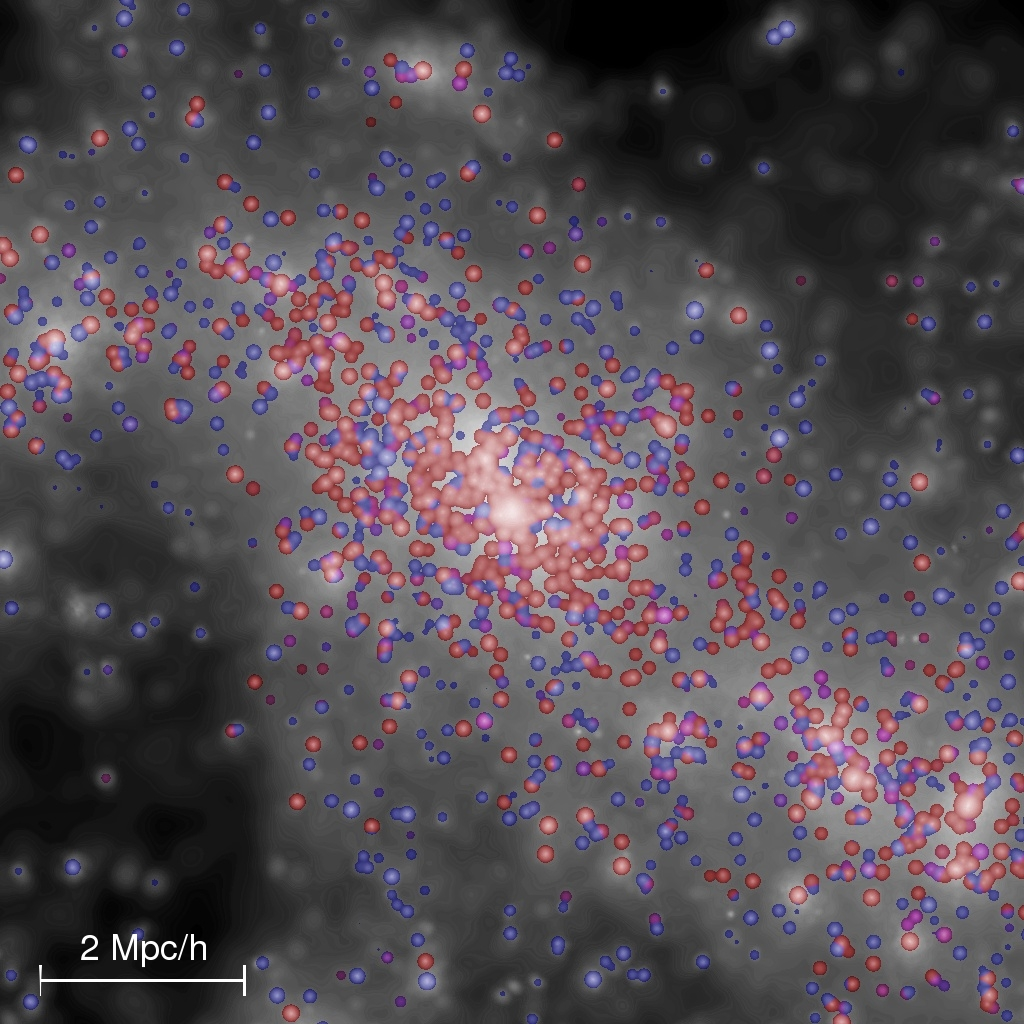
\includegraphics[width=\textwidth]{figs-swe/thesis/ms_galaxies.jpg}
        \captionsetup{justification=raggedright,singlelinecheck=false}
        \caption{CAPTION}
        \label{ms_galaxies}
    \end{subfigure}
    ~
    %% Einstein Ring Figure
    \begin{subfigure}[H]{0.375\textwidth}
        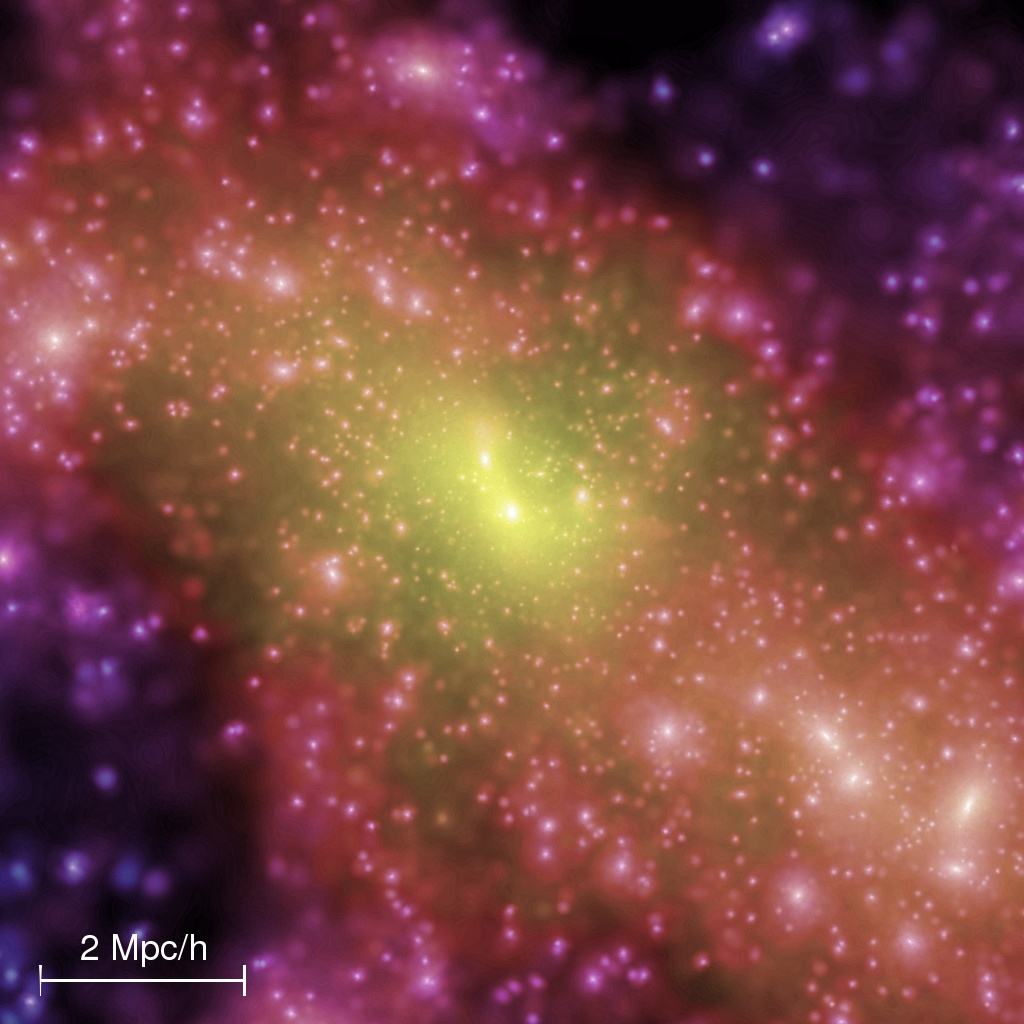
\includegraphics[width=\textwidth]{figs-swe/thesis/ms_halos.jpg}
        \captionsetup{justification=raggedright,singlelinecheck=false}
        \caption{CAPTION}
        \label{ms_halos}
    \end{subfigure}
    \caption{}
    \label{ms_compare}
\end{figure*}

%%------------------------------------------------------------------------------------------------------------------------------------------

Cosmological simulations like the Millennium Simulation (MS) demonstrate that the underlying dark matter distribution of our universe is likely breathtakingly complex; rather than a largely disordered collection of galaxies and interstellar gas, matter appears to condense into clusters and superclusters of galaxies threaded together by large filaments (pocketed) with under-dense regions called voids, as shown in Figure ??(1.a) (CITE MS). While the exact relation between the distribution of galaxies and dark matter is not known, simulations predict that early galaxies formed in the large gravitational potentials of over-dense regions of dark matter (CITE!). This suggests that, while we cannot map dark matter directly, galaxies should trace out at least some of the underlying dark matter structures (Citation!). A comparrison of the predicted galaxy and dark matter distribution from a small region of the MS is shown in Figure \ref{ms_compare}.

%However, these simulations also indicate that galaxies tend to form in the large gravitational potentials of dark matter over-dense regions of dark matter. While the exact relation between the distribution of galaxies and dark matter is not known, this m

The simplest way to model the relationship between galaxies and the dark matter distribution is by enveloping each galaxy in a spherically symmetric dark matter `halo' of a certain mass $M_h$. These halos extend far beyond the edge of the visible galaxy that they enclose, with the Milky Way's own halo estimated to have a radius of (Check and cite!). While the density profile of the halos may be complex, numerous simulations have shown that it can be well approximated locally by the Navarro-Frenk-White (NFW) profile which has the form
\begin{equation}\label{nfw_profile}
\rho_{NFW}(r)=\frac{\rho_0}{\frac{r}{R_s}\left(1+\frac{r}{R_s}\right)^2}
\end{equation}

\noindent where the constant $\rho_0$ and the scale radius $R_s$ are parameters that vary from halo to halo \cite{nfw}. However, the NFW profile is not entierly physical as the total mass diverges as the desntiy is integrated out to an infinite radius, so this work uses a truncated NFW profile called the Baltz-Marshall-Oguri (BMO) profile given by
\begin{equation}\label{bmo_profile}
\rho_{BMO}(r)=\rho_{NFW}\cdot\left(\frac{r_t^2}{r^2+r_t^2}\right)^2
\end{equation}

\noindent where $r_t$ is the truncation radius as it has been shown to be a better fit to simulated data \cite{nfw_bmo}.


%%------------------------------------------------------------------------------------------------------------------------------------------
\subsection{Filaments, Voids, and the Smooth-Component Correction} \label{scc}

The halo model only accounts for dark matter structures associated with galaxies. However, this neglects other mass structures such as the filaments and voids that can be seen in Figure (??). Modelling these features accurately would be difficult; we could try, for example, to model filaments by attaching cylinders of dark matter between massive clusters of galaxies. While an intriguing idea, rigorously testing for the appropriate filament density distributions, selection criteria, and frequency to statistically match simulations could constitute its own thesis.

% However, the mean mass density of large enough ($\sim$100 Mpc) regions should approximate the mean mass density of the universe, so for a first guess we can approximate the additional mass as a series of uniform sheets of matter a each redshift that make the total mass density of the foreground catalog equal to the mean density of the universe. This assumption can be expressed as

Instead, as the mean mass density of large enough ($\sim$100 Mpc) regions should approximate the mean mass density of the universe, we can make a `first-order' approximation by assuming that all additional mass (or absence of mass) is contained in a uniform `smooth-component' density that ensures the total mass density of any sufficiently large region equals the mean density of the universe at that redshift. This assumption can be expressed as
\begin{equation}\label{smooth_correction1}
\rho_{\text{matter}}(z)=\rho_{\text{halos}}(z)+\rho_{\text{smooth}}(z)
\end{equation}

\noindent where $z$ is the redshift and $\rho_{\text{matter}}(z)$, $\rho_{\text{halos}}(z)$, and $\rho_{\text{smooth}}(z)$ are the mean matter densities of the universe, halos, and smooth-component correction respectively. For simplicity, we rename theses quantities ${\rho_m(z)}$, ${\rho_h(z)}$, and ${\rho_s(z)}$ so that Equation \eqref{smooth_correction1} now reads as
\begin{equation}\label{smooth_correction2}
\rho_m(z)=\rho_h(z)+\rho_s(z).
\end{equation}

To solve for the desired smooth-component correction, we first need to calcualte ${\rho_m(z)}$ and ${\rho_h(z)}$ and then subtract:
\begin{equation}\label{smooth_correction2}
\rho_s(z)=\rho_m(z)-\rho_h(z).
\end{equation}

\noindent Note that, unlike the halo density, each smooth-component mass sheet at a given $z$ can have positive \textit{or} negative mass density as the halos at that redshift could happen to be in a local overdensity or underdensity.

%%------------------------------------------------------------------------------------------------------------------------------------------
\subsubsection{Calculating $\mathbf{\rho_m(z)}$:}

Using the fluid equation and equation of state (Cite), we can show that the energy density of non-relativistic matter $\varepsilon_m(z)$ evolves as
\begin{equation}\label{energy_evol}
\varepsilon_m(z)=\frac{\varepsilon_{m,0}}{a(z)^3}=\varepsilon_{m,0}(1+z)^3
\end{equation}

\noindent where $a(z)=(1+z)^{-1}$ is the cosmic scale factor (${a(0)=1}$ by convention) and a subscript of 0 means the value at the present time, or equivalently a redshift of 0. This is physically intuitive as the (mostly constant) mass is being diluted by an expanding volume. As the mass is non-relativistic, its energy density can be approximated by
\begin{equation*}\label{energy_mass}
\varepsilon_m(z)\approx\rho_m(z)c^2
\end{equation*}

\noindent and thus
\begin{equation}\label{mass_evol}
\rho_m(z)\approx\rho_{m,0}(1+z)^3.
\end{equation}

The current matter density $\rho_{m,0}$ is usually reported in literature in terms of the present matter density parameter $\Omega_{m,0}$ defined as
\begin{equation}\label{}
\Omega_{m,0}=\frac{\rho_{m,0}}{\rho_{c,0}}=\frac{8\pi G}{3H_0^2}\,\rho_{m,0}
\end{equation}

\noindent where $\rho_{c,0}=\frac{3H_0^2}{8\pi G}$ is the present critical density. Solving for $\rho_{m,0}$ gives
\begin{equation*}\label{}
\rho_{m,0}=\frac{3H_0^2}{8\pi G}\,\Omega_{m,0}
\end{equation*}

\noindent and so we may write the non-relativistic mass density of the universe as a function of redshift as
\begin{equation}\label{rho}
\rho_m(z)\approx\left(\frac{3H_0^2}{8\pi G}\,\Omega_{m,0}\right)(1+z)^3.
\end{equation}

%%------------------------------------------------------------------------------------------------------------------------------------------
\subsection*{Calculating $\mathbf{\rho_h(z)}$:}

The halo mass density $\rho_h(z)$ at a given redshift is simply the sum of the individual halo masses $M_{h,i}$ over a physical volume $dV_p$. However, we want a proper volume element that is expressed in terms of the solid angle $d\Omega$ and the redshift $dz$. To do this, we can start with the standard spherical volume element $dV=r^2drd\Omega$. However, one must be careful to (1) use proper distances, (2) account for the possibility of a curved universe, and (3) use the correct distance measure for $r$ (in this case, the angular diameter distance). From this one can infer that the proper volume element must have the form of
\begin{equation}\label{proper_element}
dV_p=d_A(z)^2dr_pd\Omega
\end{equation}

\noindent where $d_A(z)$ is the angular diameter distance and the subscript $p$ denotes proper distance. When the angular diameter distance $d_A(z)$ is multiplied by an angle (i.e. $d_A(z)d\theta$ and $d_A(z)d\phi$), it gives an approximation of the proper distance between two objects at the same redshift. $d_A(z)$ can be expressed in terms of the transverse comoving distance $d_M(z)$,
\begin{equation}\label{angular2transverse}
d_A(z)=a(z)d_M(z)=\frac{d_M(z)}{1+z}
\end{equation}

\noindent which is the comoving analog of $d_A(z)$. The transverse comoving distance depends on the assumed cosmology of the universe and takes the form of
\begin{equation}\label{comoving_transverse}
d_M(z)=\left\{
     \begin{array}{lr}
       d_H/\sqrt{\Omega_k}\sinh\left[\sqrt{\Omega_k}d_C(z)/d_H\right] & : \Omega_k>0\\
       d_C(z) & : \Omega_k=0\\
       d_H/\sqrt{|\Omega_k|}\sin\left[\sqrt{|\Omega_k|}d_C(z)/d_H\right] & : \Omega_k<0
     \end{array}
   \right.
\end{equation}

\noindent where $d_H=c/H_0$ is the Hubble distance, $\Omega_k$ is the curvature parameter ($\Omega_k=0$ for a flat universe), and $d_C(z)$ is the line-of-sight (LOS) comoving distance given by
\begin{equation}\label{comoving_distance}
d_C(z)=d_H\int_0^z\frac{dz^\prime}{E(z^\prime)}
\end{equation}

\noindent where $E(z)$ is the dimensionless Hubble parameter
\begin{equation}\label{dim_hubble_parameter}
E(z)=\sqrt{\Omega_m(1+z)^3+\Omega_k(1+z)^2+\Omega_\Lambda}.
\end{equation}

\noindent Substituting Equation \eqref{angular2transverse} into \eqref{proper_element} leads to
\begin{align}\label{temp_solution}
dV_p&=d_a(z)^2dr_pd\Omega\nonumber\\
&=\frac{d_m(z)^2}{(1+z)^2}dr_pd\Omega
\end{align}

\noindent and so all that remains is to express $dr_p$ in terms of $dz$.

As the LOS proper distance between two objects $r_p(z)$ is related to the LOS comoving distance $d_C(z)$ by
\begin{equation}\label{physical2comoving}
r_p(z)=a(z)d_C(z)=\frac{d_H}{1+z}\int_0^z\frac{dz^\prime}{E(z^\prime)},
\end{equation}

\noindent it follows that that an infinitesimal proper displacement $dr_p$ is given by
\begin{equation}\label{physical2comoving_inf}
dr_p=\frac{d_H}{E(z)(1+z)}dz.
\end{equation}

\noindent Combining this result with Equation \eqref{temp_solution} leads to the desired proper volume element given by
\begin{equation}\label{pvolume_element}
dV_p=\frac{d_Hd_M(z)^2}{E(z)(1+z)^3}dzd\Omega.
\end{equation}

The proper volume is found by integrating the above volume element over the solid angle $d\Omega$ and the desired $dz$ range, so the halo density $\rho_h(z)$ is then given by

\begin{align}\label{rho_h}
\rho_h(z)&=\frac{\sum_i M_{h,i}}{V(z)}\nonumber\\
&=\sum_i M_{h,i}\cdot\left(d_H\int\frac{d_M(z^\prime)^2}{E(z^\prime)(1+z^\prime)^3}dz^\prime d\Omega\right)^{-1}.
\end{align}

\noindent and the smooth-component correction is simply the difference between Equations \eqref{rho} and \eqref{rho_h}.

% With this, the proper volume of olume of the lightcone a given grid slice at redshift $z$ in a foreground catalog centered at ($\theta,\phi$) by integrating the above volume element over the solid angle $d\Omega$ and $\Delta z$ range of the redshift slice:
% \begin{align}
% V(z)&=\int_{V_z}dV_p\\ \nonumber
% &=d_H\int_\Omega\int_{z-\frac{\Delta z}{2}}^{z+\frac{\Delta z}{2}} \frac{d_M(z^\prime)^2}{E(z^\prime)(1+z^\prime)^3}dz^\prime d\Omega.
% \end{align}

%%------------------------------------------------------------------------------------------------------------------------------------------
\subsection{Gravitational Lensing} \label{grav_lensing}

%%------------------------------------------------------------------------------------------------------------------------------------------
%% Ellipticity Orientation Figure
\begin{figure*}
    \centering
    \begin{subfigure}[H]{0.415\textwidth}
        \includegraphics[width=\textwidth]{figs-swe/thesis/ellipse_orientations.png}
        \captionsetup{justification=raggedright,singlelinecheck=false}
        \caption{The shape of a galaxy image for various ellipticity components $\varepsilon_1$ and $\varepsilon_2$ on the $x$ and $y$-axes respectively. Taken from \cite{schneider}.}
        \label{ellipses}
    \end{subfigure}
    ~
    %% Einstein Ring Figure
    \begin{subfigure}[H]{0.425\textwidth}
        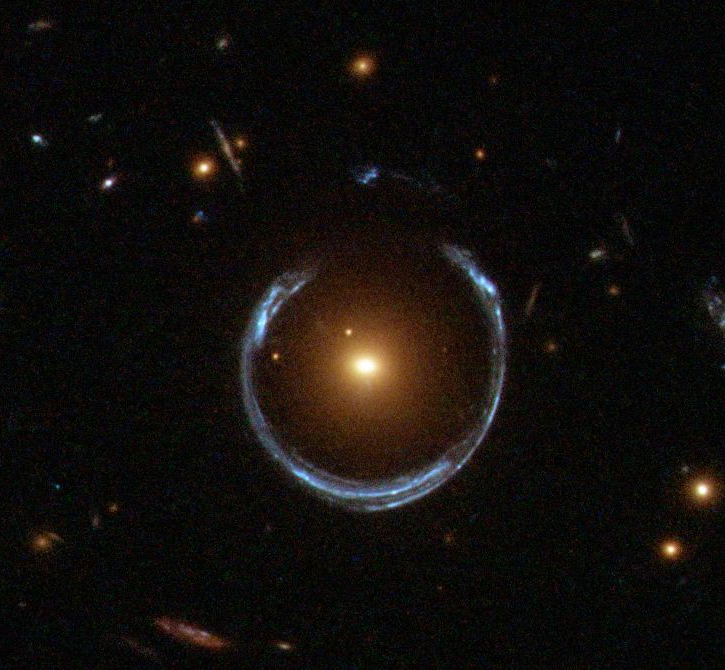
\includegraphics[width=\textwidth]{figs-swe/thesis/einstein_ring.png}
        \captionsetup{justification=raggedright,singlelinecheck=false}
        \caption{An image of the luminous red galaxy LRG 3-757 along with a strongly lensed background galaxy, called the `Cosmic Horseshoe' \cite{einstein_ring}.}
        \label{einstein_ring}
    \end{subfigure}
    \caption{}
\end{figure*}
%%------------------------------------------------------------------------------------------------------------------------------------------

While dark matter does not absorb or emit light, it does interact with light indirectly through gravitational lensing. The presence of matter curves spacetime locally which causes light to follow curved paths called geodesics. The deviation in path is usually negligable, but can be significant in regions containing clusters of galaxies and their massive dark matter halos. By observing how the magnitudes and shapes of distant galaxies are distorted when travelling through regions of matter, we can infer the masses of the dark matter halos and reconstruct the hidden dark matter mass distribution. A simplified cartoon of this process is shown in Figure ??, as well as a diagram defining the necessary angles and distances in Figure ??.

%%------------------------------------------------------------------------------------------------------------------------------------------
%% Gravitational Lensing Diagram
% \begin{figure*}
%     \centering
%     \begin{subfigure}[H]{0.4\textwidth}
%         \includegraphics[width=\textwidth]{figs-swe/thesis/lens_cartoon.png}
%         \captionsetup{justification=raggedright,singlelinecheck=false}
%         \caption{CAPTION}
%         \label{lens_cartoon}
%     \end{subfigure}
%     ~
%     %% Einstein Ring Figure
%     \begin{subfigure}[H]{0.4\textwidth}
%         \includegraphics[width=\textwidth]{figs-swe/thesis/lens_diagram.png}
%         \captionsetup{justification=raggedright,singlelinecheck=false}
%         \caption{CAPTION}
%         \label{lens_diagram}
%     \end{subfigure}
%     \caption{}
% \end{figure*}
%%------------------------------------------------------------------------------------------------------------------------------------------

A full mathematical treatment of the gravitational lensing of galaxies due to the gravitational fields of massive objects requires general relativity (see \cite{modern_cosmology} for details). However, the important results can be summarized as follows. Foreground mass distorts the image of a background galaxy in two distinct ways: The image is magnified and sheared tangentially about the foreground mass, making it more elliptical. The magnification of the image is determined by the convergence $\kappa$ defined by
\begin{equation}\label{convergence}
\kappa(\vec{\theta})=\frac{\sum(\vec{r},z_l)}{\sum_{cr}(z_l,z_s)}
\end{equation}

\noindent where $\sum(\vec{r},z_l)$ is the projected surface mass density of the lensing mass and $\sum_{cr}(z_l,z_s)$ is the critical surface density for a given source redshift $z_s$ and lens redshift $z_l$ (Citation). The shearing of the source is most often described by the complex shear $\gamma$ defined to be
\begin{equation}\label{complex_shear}
\gamma=\gamma_1+i\gamma_2=|\gamma|\,e^{2i\varphi}
\end{equation}

\noindent where $|\gamma|$ is the magnitude of the shear and $\varphi$ is the orientation of the shear. While the intrinsic ellipticities of source galaxies are randomly oriented near the foreground mass before lensing, they will be systematically more aligned with the shear field after lensing.% Figure (??) demonstrates this process visually.

However, usually the quantity of interest in lensing calculations is the reduced shear, defined as
\begin{equation}\label{reduced_shear}
g=\frac{\gamma}{1-\kappa}.
\end{equation}

\noindent Then using the thin lens approximation for the lensing of a background source of intrinsic ellipticity $\varepsilon_i$ by foreground mass at a point with reduced shear $g$, the lensed ellipticity $\varepsilon$ is given by
\begin{equation}\label{lensing}
 \varepsilon = \begin{dcases}
      \frac{\varepsilon_i+g}{1+g^*\varepsilon_i} & : |g|\leq1 \\[0.75em]
       \frac{1+g\varepsilon_i^*}{\varepsilon^*+g^*} & : |g|>1
   \end{dcases}
\end{equation}

\noindent where an asterisk denotes the complex conjugate \cite{schneider}. The behavior of the distortion relies strongly on the magnitude of $g$; the
effect is called \textit{strong} lensing if $|g|\gtrapprox1$ and \textit{weak} lensing if $|g|\ll1$. The effects of strong lensing can be quite dramatic, distorting sources into large arcs, multiple images, or even an Einstein ring as shown in Figure \ref{einstein_ring}.

While strong lenses are rare, as the alignment of the source and foreground mass must be nearly perfect, \textit{all} sources are weakly lensed when traveling through foreground halos. The effect is small, usually an ellipticity distortion of only a few percent, but can be detected locally by averaging the ellipticities of all sources in a small region. As the orientations of the sources should be random, it would be expected that
$$\left<\varepsilon\right>=0.$$

\noindent However, as sources in the same small region are sheared in (approximately) the same way, this implies that
\begin{equation}
\left<\varepsilon\right>\approx g.
\end{equation}

 \noindent Finally as in the weak lensing regime ${\kappa\ll1}$ and ${|\gamma|\ll1}$, it follows that
 \begin{equation}
 \gamma\approx g\approx\left<\varepsilon\right>
 \end{equation}

 \noindent which provides a method of detecting the shear observationally.

 The analytical form of the convergence and shear contribution from a BMO-profile is quite messy, but is derived and explained in detail in (Cite Phil's paper!!). Calculating the lensing contribution of the smooth-component correction is much simpler; the projected surface mass density at at given redshift is found by integrating $\rho_s(z)$ over a sufficiently small $dz$ interval, and then the mass sheet's convergence is found using Equation \eqref{kappa}. There is no shear contribution as a uniform sheet of mass causes only magnification due to the mass sheet degeneracy (CITE!). However, Equation \eqref{lensing} shows that the lensed ellipticities depend on the \textit{reduced} shear, which does depend on the additional convergence terms resulting from the smooth-component correction.

%%------------------------------------------------------------------------------------------------------------------------------------------
\subsection{Galaxies as Ellipses} \label{galaxies_as_ellipses}

To calculate the lensed ellipticities in the previous section, galaxies must first be translated from pixel intensities into elliptical representations of the galaxies. This is not always possible for galaxies are diverse in type and shape and not all are well approximated by ellipses. However for this thesis, all galaxy ellipticities are simulated so this issue is avoided. For a more thorough analysis of measuring image ellipticities, see Schneider (2003) \cite{schneider}.

Consider a galaxy image that can be well approximated as an ellipse at an angle $\phi$ above an arbitrary reference line. The galaxy's complex ellipticity is defined to be
\begin{equation}\label{complex_ellipticity}
\varepsilon=\varepsilon_1+i\varepsilon_2=|\varepsilon|\,e^{2i\phi}
\end{equation}

\noindent where the magnitude of the galaxy's ellipticity $|\varepsilon|$ is defined as
\begin{equation}
|\varepsilon|=\frac{1-r}{1+r}
\end{equation}

\noindent and $r\leq1$ is the ratio of the semi-minor and semi-major axes of the ellipse. This compact notation combines the eccentricity and orientation of the ellipse into a single object. A plot from Schneider (2003) \cite{schneider} showing the shape of elliptical galaxies for various values of $\varepsilon_1$ and $\varepsilon_2$ is shown in Figure \ref{ellipses}.

There are many complications to using this scheme in practice, most notably the multiplicative bias resulting from the smearing of galaxy images by the observational point spread function (PSF) \cite{multiplicative_bias}. While the effects of a PSF can be complex, in general it causes galaxy images to appear less elliptical than they truly are. To account for this in generated galaxy images, a multiplicative bias parameter $M$ is often used to lessen the intrinsic ellipticity using
\begin{equation}\label{mult_bias}
\varepsilon_{\text{obs}}=M\cdot\varepsilon_{\text{int}}
\end{equation}

\noindent where $\varepsilon_{\text{int}}$ is the generated intrinsic ellipticity of the image and $\varepsilon_{\text{obs}}$ is the ellipticity that would be recorded by a detector.


%%------------------------------------------------------------------------------------------------------------------------------------------
\subsection{Correlation Functions} \label{corr_functions}

If all galaxies were spherical, then the measurement of their ellipticities would give an exact description of the lensing done by foreground mass structures. Unfortunately, the intrinsic ellipticities of background galaxies contribute significant noise as we do not know how any individual galaxy ellipticity has been altered by lensing. However as two sources lensed by the same foreground mass will have their ellipticities distorted (in a similar way), their lensed ellipticities should be correlated regardless of intrinsic orientation. The average correlation of a sufficient number of galaxy pairs should overcome the noise and lead to a detectable signal. Importantly, this implies that \textit{the correlation of galaxy ellipticities is a probe of the underlying dark matter mass distribution} (Citation!).

The mathematical tool that measures the average correlation as a function of separation distance between two galaxies is called the ellipticity-ellipticity ($\varepsilon$-$\varepsilon$) correlation function. A quick overview of this function is given below, but readers that are unfamiliar with correlation functions in the context of cosmology or want a visual aid should see Appendix (??).

Given two galaxies with ellipticities $\varepsilon_i$ and $\varepsilon_j$ whose orientation is offset by polar angle $\alpha$, the tangential and cross-component components of the ellipticities, $\varepsilon_t$ and $\varepsilon_\times$ respectively, for each are defined as
\begin{align}
\varepsilon_{k_t}&=-\operatorname{Re}\left(\varepsilon_k e^{-2i\alpha}\right),\\
\varepsilon_{k_\times}&=-\operatorname{Im}\left(\varepsilon_k e^{-2i\alpha}\right).
\end{align}

\noindent Instead of using the autocorrelation and cross-correlation of these quantities, it turns out to be more convenient to define the combinations

\begin{align}\label{gg_corr_def}
\xi_\pm(\Delta\theta)&=\left<\varepsilon_{i_t}(\vec{\theta})\varepsilon_{j_t}(\vec{\theta}+\vec{\Delta\theta})\right>\pm\left<\varepsilon_{i_\times}(\vec{\theta})\varepsilon_{j_\times}(\vec{\theta}+\vec{\Delta\theta})\right>\\
\xi_\times(\vec{\Delta\theta})&=\left<\varepsilon_{i_t}(\vec{\theta})\varepsilon_{j_\times}(\vec{\theta}+\vec{\Delta\theta})\right>
\end{align}

\noindent where $\vec{\theta}$ is the position vector of the first galaxy and $\Delta\vec{\theta}$ is the angular separation vector between the pair of galaxies \cite{schneider}. Gravitational lensing shears ellipticities tangentially, so $\xi_\times(\Delta\theta)$ should vanish with enough galaxies and therefore is a useful estimate of the bias. (\textcolor{red}{Why is $\xi_-$ expected to be zero?}), which leaves $\xi_+(\Delta\theta)$ as the desired probe of lensing mass.

As galaxies will only be lensed by the same foreground mass at relatively small separation distances, the $\varepsilon$-$\varepsilon$ correlation function decreases sharply as the separation increases. If the distribution of intrinsic galaxy ellipticities is indeed random, then their $\varepsilon$-$\varepsilon$ correlation function should be essentially zero across all separation scales. 

A similar statistical measure often used in ... is the galaxy-mass correlation function, which measures ... and is defined as
\begin{equation}\label{ng_corr_def}
\xi=
\end{equation}

\noindent where...


%%==========================================================================================================================================
\section{Pangloss: Line of Sight Mass Reconstructions} \label{pangloss}

%%------------------------------------------------------------------------------------------------------------------------------------------
%% Pangloss Cartoon
\begin{figure*}
    \centering
    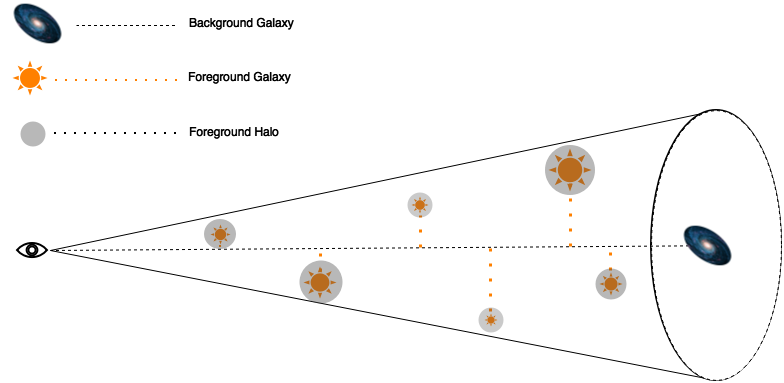
\includegraphics[width=0.85\textwidth]{figs-swe/thesis/pangloss_cartoon.png}
    \captionsetup{justification=raggedright,singlelinecheck=false}
    \caption{A cartoon model of how the \texttt{Pangloss} framework uses a dark matter halo model to reconstruct the foreground mass along the line of sight of a background source galaxy. A `lightcone' centered at a background source is constructed with radius $R_L$ and populated with all foreground galaxies contained in this volume. Each foreground object has an attached dark matter halo and physical distance to the line of sight (dashed line). The shear and convergence along the line of sight contributed by each halo is calculated using \cite{lensing_calc}, and the predicted ellipticity is determined using the sum of these contributions and Equation \eqref{lensing}.}
    \label{pangloss_cartoon}
\end{figure*}
%%------------------------------------------------------------------------------------------------------------------------------------------

To infer foreground dark matter mass structures using weak gravitational lensing, first a model of the relationship between foreground galaxies and the foreground dark matter must be established and robustly tested to see if, statistically, it makes the same lensing predictions of background sources as the true underlying dark matter structure. To do this, I built upon the publicly available \texttt{Pangloss}\footnote{\label{note1}https://github.com/drphilmarshall/Pangloss} framework used in Collett et al. \cite{collett_marshall} to reconstruct all the
mass along the lines of sight of generated background galaxies in the MS using a halo model with smooth-component correction. The lensing contribution of each halo is calculated, and the total lensing of the background galaxy is the sum of each halo contribution. The implementation of this process is detailed in the following sections.


%%------------------------------------------------------------------------------------------------------------------------------------------
\subsection{Model Assumptions} \label{assumptions}
While \texttt{Pangloss} may be used more generally, the present analysis makes some additional strong assumptions to simplify the problem for a first attempt at making weak lensing predictions:

\begin{enumerate}
\item The dark matter mass distribution can be approximated by spherically symmetric BMO halo profiles attached to each galaxy, along with a smooth-component correction.
\item The stellar mass of the foreground galaxy is negligible for lensing calculations.
\item The mass of the dark matter halo of each foreground galaxy is known.
\item A spectroscopic redshift of each foreground galaxy is known.
\end{enumerate}

Testing the first assumption is the main goal of this paper. The second assumption is reasonable as it is estimated that dark matter halos are on average 1-2 orders of magnitude more massive than the host galaxy \cite{smhr}. Clearly the third assumption will never be true for any observational data. However, this allows for a best-case estimate of how well the \texttt{Pangloss} framework \textit{could} predict weak lensing effects given all possible information. This assumption can be relaxed by sampling a dark matter halo mass from an assumed stellar mass - halo mass relation. The fourth assumption is also unrealistic as most galaxies in sky surveys only have a less-reliable photometric redshift due to time constraints, but this again allows for a best-case estimate. This assumption could be relaxed by instead using photometric redshifts, adding random noise, and repeating the upcoming analysis on many realizations of the photometric redshifts.


%%------------------------------------------------------------------------------------------------------------------------------------------
\subsection{The Millennium Simulation} \label{ms}
\texttt{Pangloss} cannot be used to make dark matter mass maps using existing galaxy catalogs until it is tested on a simulated universe with known dark matter structure to determine how accurately and precisely it predicts the lensing of background sources. For this purpose, \texttt{Pangloss} was tested on galaxy catalogs from the Millennium Simulation, an N-body simulation consisting of over 10 billion dark matter `particles' each representing a billion solar masses and populated with about 20 million galaxies \cite{millennium_simulation}. The simulation contains baryonic and dark matter structure believed to be similar to our own universe, and uses cosmological parameters from WMAP 1\textsuperscript{st}-year data analysis which assumed a matter density of $\Omega_m=0.25$, a dark energy density of $\Omega_\Lambda=0.75$, and a Hubble constant of $H_0=73$ km$\,$s$^{-1}\,$Mpc$^{-1}$ (Cite). From the work of Hilbert et al. \cite{ray_tracing}, high resolution maps of the ray-traced shear and convergence of galaxy sources at $z=1.3857$ are publicly available. From these maps, an estimate of the `true' lensing of background galaxy ellipticities when traveling through the foreground mass of the Millennium Simulation can be calculated using Equation \eqref{lensing}.


%%------------------------------------------------------------------------------------------------------------------------------------------
\subsection{Generating Background Galaxies}
With the (0,0,0,0) catalog of MS foreground galaxies chosen, a set of ?? background galaxies over a field of ?? arcmin$^2$ was generated, with density 10 per arcmin$^2$. The intrinsic orientation of each galaxy was sampled from a uniform distribution as, without lensing, there should be no preferred orientation due to the assumption of an isotropic universe. The magnitude of the galaxy ellipticities was sampled from a normal distribution with a standard deviation of 0.2, but any ellipticities with magnitude greater than one were re-sampled. Random ellipticity noise was sampled from a normal distribution with a standard deviation of 0.1 and added to the intrinsic ellipticities. Finally, each ellipticity was multiplied by $M=0.9$ to account for a multiplicative bias of 10\%.


%%------------------------------------------------------------------------------------------------------------------------------------------
\subsection{Creating Lightcones}

While ideally all foreground mass in a field would be considered when predicting the weak lensing of a background galaxy, it is computationally prohibitive to do so. Instead, all foreground halos contained within a `lightcone' centered along the line of sight to the source and extending out to a chosen lightcone radius $R_L$ were considered when calculating the lensing contributions for the background source. A cartoon model of this process is shown in Figure \ref{pangloss_cartoon}. Unless otherwise specified, experiments in this paper used a radius of 6 arcminutes and halo truncation scale of five times the virial radius.

To calculate the convergence and shear contribution of each halo, the physical distance from the halo to the line of sight was needed. To increase the speed of distance calculations, the foreground halo redshifts were first binned to a grid of 100 equally-sized redshift bins $\Delta z=0.013857$ from $z=0$ to the sourced redshift of $z=1.3857$, and then converted to physical distances using the cosmology defined by the Millennium Simulation.

\subsection{Assigning Relevance to Halos}

Not all foreground halos are equally relevant to the lensing calculation. To add a significant contribution to the combined shear and convergence, a halo must be massive, close to the line of sight, or preferably both. McCully et al. (Cite) derived that the correct metric for determining the relevance of a given foreground halo to the overall lensing calculation to be given by
\begin{equation}\label{relevant}
Rel(M_h,R)\propto\frac{M_h}{R^3}
\end{equation}

\noindent where $M_h$ is the halo mass and $R$ is the distance from the halo to the line of sight. Numerical values are assigned by comparing a halo's individual $M_h$ and $R$ to a threshold $M_T$ and $R_T$:
\begin{equation}\label{relevant_thresh}
Rel(M_h,R)=\frac{(M_h/M_T)}{(R/R_T)^3}.
\end{equation}

In this work, the threshold values used are $M_T=10^{12}M_\odot$ and $R_T=10$ kpc. The relevance distribution for one background catalog realization with ?? foreground halos in a lightcone of radius ?? arcminutes is shown in Figure ??. As expected, there are very few massive halos along the line of sight and therefore only a small percentage of foreground halos should have a high relative contribution to the predicted lensing quantities. This encouraged the intended analysis on lightcones with all halos and those with only a small subset of the most relevant halos to compare the results and see if the computational time saved by using only the most relevant halos was worth the loss in prediction accuracy.

%%------------------------------------------------------------------------------------------------------------------------------------------
%% Relevance Distribution of all Halos
\begin{figure}
    \centering
    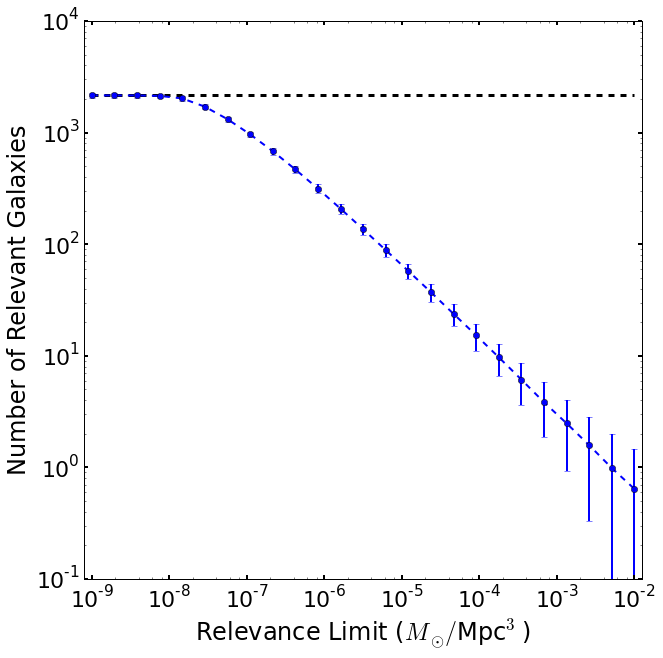
\includegraphics[width=0.5\textwidth]{figs-swe/thesis/relevance_distribution.png}
    \captionsetup{justification=raggedright,singlelinecheck=false}
    \caption{CAPTION}
    \label{fig:rel_dist}
\end{figure}
%%------------------------------------------------------------------------------------------------------------------------------------------


%%------------------------------------------------------------------------------------------------------------------------------------------
\subsection{Calculating the Smooth-Component Correction} \label{calc_scc}

%%------------------------------------------------------------------------------------------------------------------------------------------
%% Smooth-Component Correction Diagram
\begin{figure}
    \centering
    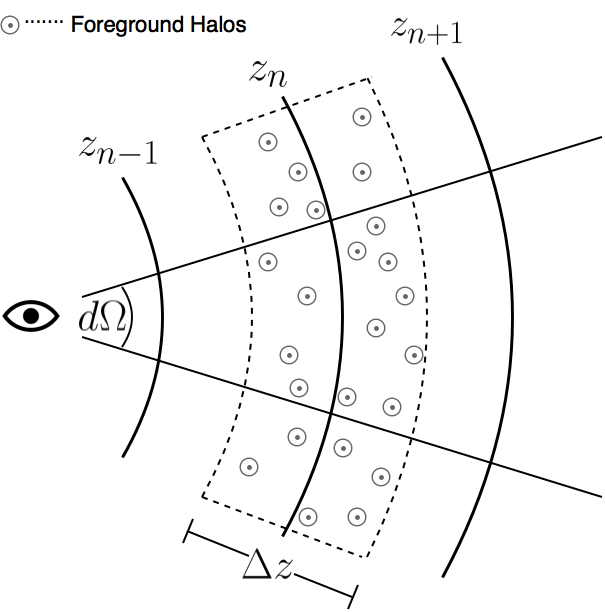
\includegraphics[width=0.5\textwidth]{figs-swe/thesis/smooth_correction.png}
    \captionsetup{justification=raggedright,singlelinecheck=false}
    \caption{CAPTION}
    \label{fig:scc}
\end{figure}
%%------------------------------------------------------------------------------------------------------------------------------------------

As discussed in Section \ref{scc}, the halo model does not account for additional mass structures such as filaments. To apply the smooth-component correction to \texttt{Pangloss}, the mean mass density $\rho(z)$ and halo density $\rho_h(z)$ had to be calculated at each of the 100 redshift bins. For $\rho_h(z)$, this was done by summing all halo masses $M_{h,i}$ in a given redshift bin and integrating Equation \eqref{pvolume_element} from ${z-\Delta z/2}$ to ${z+\Delta z/2}$, except for the boundary bins, and multiplying by the solid angle of a cone ${\Omega=2\pi(1-\cos R_L)}$. Once $\rho_h(z)$ had been calculated for each redshift slice, the projected surface mass density was found by integrating over the redshift interval,
\begin{align}\label{surface_density} 
\sum(z)&=\int_{z-\frac{\Delta z}{2}}^{z+\frac{\Delta z}{2}} \rho_s(z)\,dz\nonumber\\
&=\int_{z-\frac{\Delta z}{2}}^{z+\frac{\Delta z}{2}} \rho(z)-\rho_h(z)\,dz,
\end{align}

\noindent and the convergence contribution of the mass sheet was calculated using Equation \eqref{convergence} with ${z_l=z}$ and ${z_s=1.3857}$. The corrected total convergence for a given background source is simply the sum of the halo contributions and the smooth-component contributions. There is no additional shear produced by a uniform sheet of mass (citation!), but the corrected reduced shear is now calculated using the corrected total $\kappa$ in Equation \eqref{reduced_shear}. A diagram of this process is shown in Figure \ref{fig:scc}.

The volume and projected surface mass densities of each redshift slice are shown in Figures \ref{fig:volume_densities} and \ref{fig:surface_densities} respectively. In each plot, the halo density at each redshift slice is plotted in green, the smooth-component density in blue, and universe mean density in black, and a histogram of the galaxies per bin is shown in the background. In most redshift bins, the halo density is one to two orders of magnitude lower than than the universe mean density leading to a smooth-component density very close to that of the mean density. This seems to be in opposition to Pache et al. (year) \cite{pache} who found that halos constituted ??\% of simulation mass in ??. However, all mass densities are far below the critial density, plotted in red, and so well within the weak-lensing regime. The convergence distribution of each halo and 100 smooth-components is plotted in Figure \ref{fig:kappa_dist}.
%%------------------------------------------------------------------------------------------------------------------------------------------
%% Surface and Volume densities for smooth-component correction redshift slices
\begin{figure*}
    \centering
    % Volume
    \begin{subfigure}[H]{0.49\textwidth}
        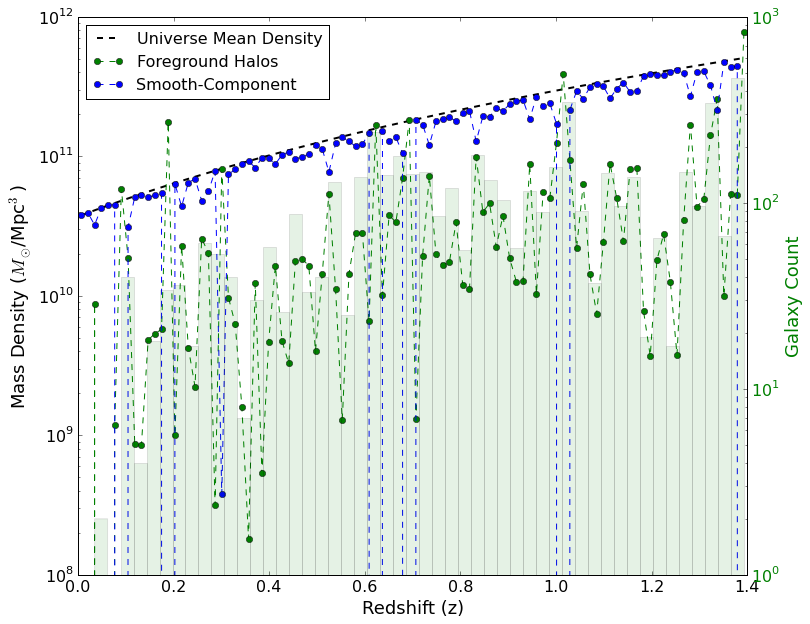
\includegraphics[width=\textwidth]{figs-swe/thesis/vol_densities.png}
        \captionsetup{justification=raggedright,singlelinecheck=false}
        \caption{CAPTION}
        \label{fig:volume_densities}
    \end{subfigure}
    ~
    % Surface
    \begin{subfigure}[H]{0.49\textwidth}
        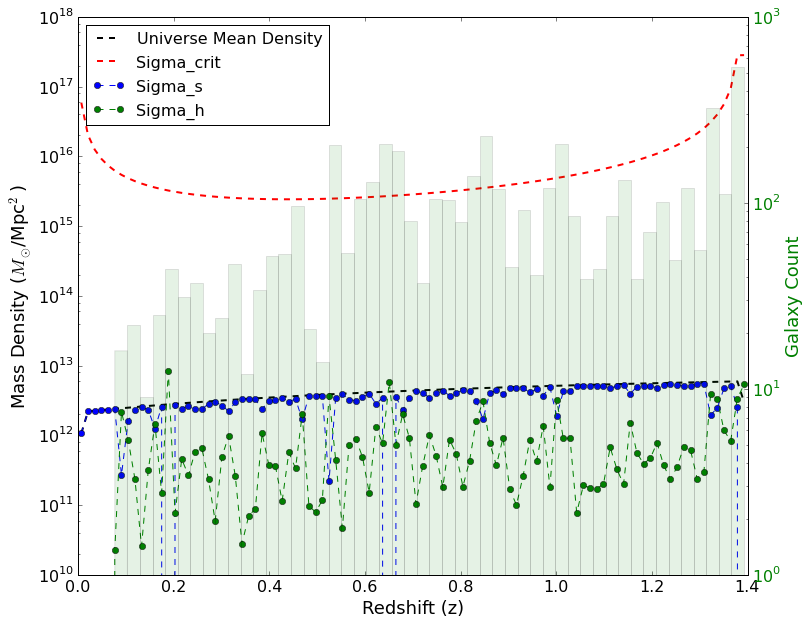
\includegraphics[width=\textwidth]{figs-swe/thesis/surf_densities.png}
        \captionsetup{justification=raggedright,singlelinecheck=false}
        \caption{CAPTION}
        \label{fig:surface_densities}
    \end{subfigure}
    \caption{}
\end{figure*}
%%------------------------------------------------------------------------------------------------------------------------------------------

%%------------------------------------------------------------------------------------------------------------------------------------------
%% Kappa Contributions of S.C.C.
\begin{figure}
    \centering
    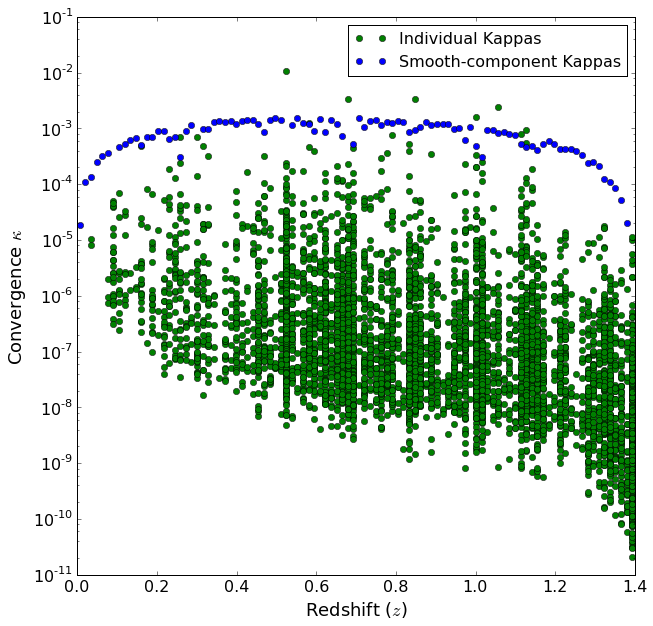
\includegraphics[width=0.475\textwidth]{figs-swe/thesis/kappa_distribution.png}
    \captionsetup{justification=raggedright,singlelinecheck=false}
    \caption{CAPTION}
    \label{fig:kappa_dist}
\end{figure}
%%------------------------------------------------------------------------------------------------------------------------------------------


%%------------------------------------------------------------------------------------------------------------------------------------------
\subsection{Line of Sight Lensing Predictions}

Using the physical separation distance and halo mass, the shear and convergence contribution of a single foreground halo is calculated using methods described in Section \ref{grav_lensing} (see Wright and Brainerd \cite{lensing_calc} for far more detail). The total convergence and shear along the LOS of the lightcone is simply the sum of the convergence and shear contributions of each halo contained in the lightcone, as well as the additional convergence terms from the smooth-component correction. The \texttt{Pangloss} predicted lensed source ellipticity is then calculated using Equation \eqref{lensing}.


%%==========================================================================================================================================
\section{Checking the Pangloss Model} \label{check}

%%------------------------------------------------------------------------------------------------------------------------------------------
%% Pangloss Lightcone Data Plots
\begin{figure*}
    \centering
    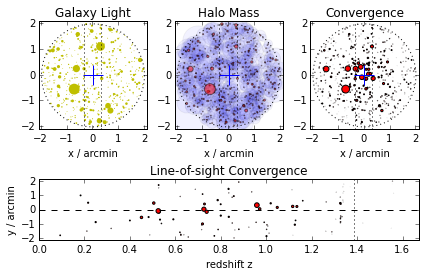
\includegraphics[width=0.75\textwidth]{figs-swe/thesis/lightcone_plots.png}
    \captionsetup{justification=raggedright,singlelinecheck=false}
    \caption{CAPTION}
    \label{fig:lightcone}
\end{figure*}
%%------------------------------------------------------------------------------------------------------------------------------------------

Using the presented methodology, ??? background galaxies in a ??? arcmin$^2$ subset of the (0,0,0,0) Millennium Simulation foreground catalog were generated and lensed by both the ray-traced shear and convergence maps as well as the \texttt{Pangloss} framework. With a lightcone radius of ?? arcminutes, the lightcones contained an average of ${??\pm??}$ foreground halos. Both sets of lensed ellipticities were characterized with correlation functions, as well as the intrinsic ellipticities of the sources before lensing.

Figure \ref{fig:lightcone} displays different views an example lightcone where the foreground halos are plotted as circles whose size are proportional to their galaxy brightness (top left), angular size (top center), convergence contributions (top right), and halo mass (bottom). Figure \ref{fig:subplots} shows a few examples of mass structures in the foreground catalog along with the ray-traced convergence (plotted in inverse greyscale) and shear maps (plotted as red ellipticity sticks) from \cite{ray_tracing}. 

Instead of comparing the ray-traced and \texttt{Pangloss} predicted ellipticities for individual galaxies, the lensing is characterized globally with correlation functions. As described in section \ref{corr_functions}, the ellipticity-ellipticity correlation function measures how correlated the ellipticities of pairs of galaxies are as a function of separation distance, while the galaxy-mass correlation function measures the correlation of lensed ellipticities around foreground halos as a function of separation distance. Both correlation functions are used in this work to estimate how well the \texttt{Pangloss} framework models weak lensing by dark matter structures and are computed using the publicly available \texttt{TreeCorr} module written by Mike Jarvis\footnote{https://github.com/rmjarvis/TreeCorr}. Note that the ellipticity-ellipticity correlation function definition used in \texttt{TreeCorr} is slightly different than that used in most of the literature; for a derivation of the connection between Jarvis's definition and the more common Schneider definition \cite{schneider}, see Appendix (??).

%%------------------------------------------------------------------------------------------------------------------------------------------
%% Two or Three subplots of foreground/background/shear/kappa maps
% \begin{figure*}
%     \centering
%     % Volume
%     \begin{subfigure}[H]{0.415\textwidth}
%         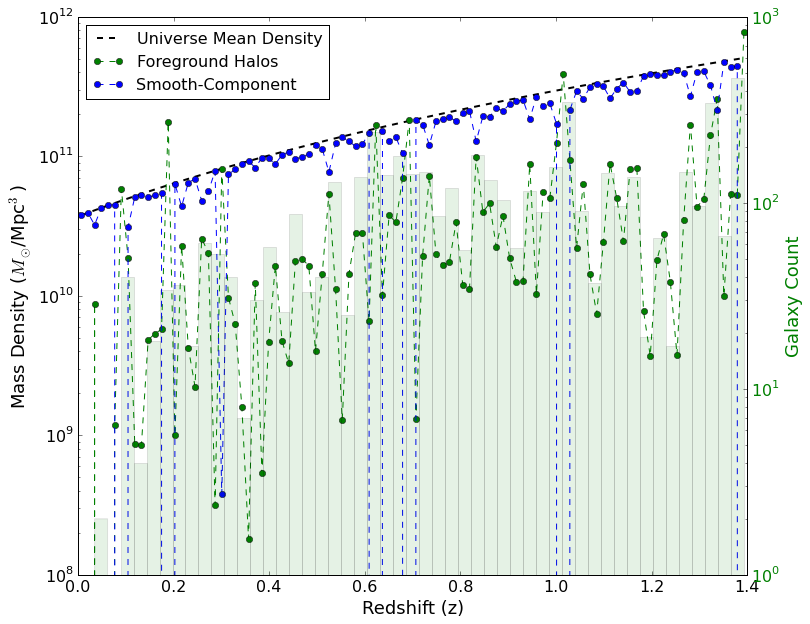
\includegraphics[width=\textwidth]{figs-swe/thesis/vol_densities.png}
%         \captionsetup{justification=raggedright,singlelinecheck=false}
%         \caption{CAPTION}
%         \label{fig:volume_densities}
%     \end{subfigure}
%     ~
%     % Surface
%     \begin{subfigure}[H]{0.425\textwidth}
%         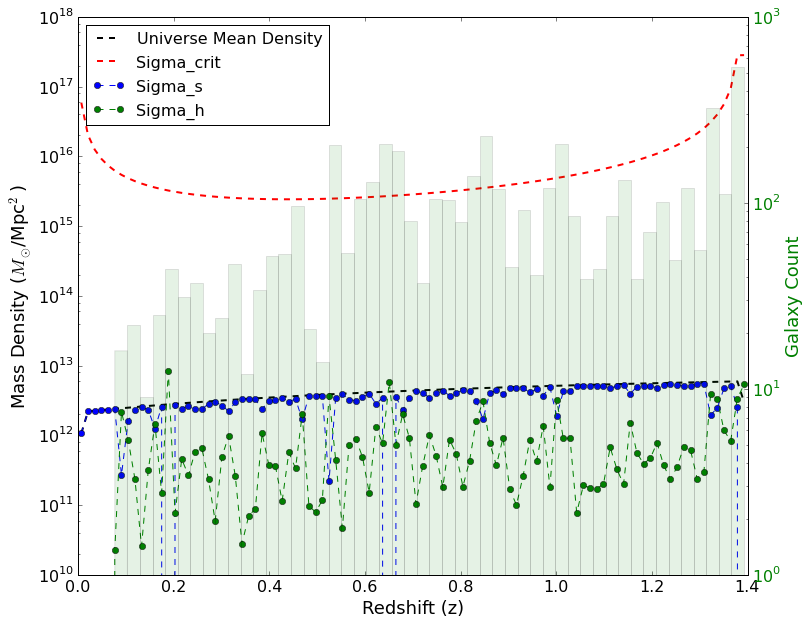
\includegraphics[width=\textwidth]{figs-swe/thesis/surf_densities.png}
%         \captionsetup{justification=raggedright,singlelinecheck=false}
%         \caption{CAPTION}
%         \label{fig:surface_densities}
%     \end{subfigure}
%     \caption{}
%     \label{fig:subplots}
% \end{figure*}
%%------------------------------------------------------------------------------------------------------------------------------------------


%%------------------------------------------------------------------------------------------------------------------------------------------
\subsection{Ellipticity-Ellipticity Correlation Function}

%%------------------------------------------------------------------------------------------------------------------------------------------
% Ellipticity-Ellipticity Correlation
\begin{figure}
    \centering
    \begin{subfigure}{0.475\textwidth}
        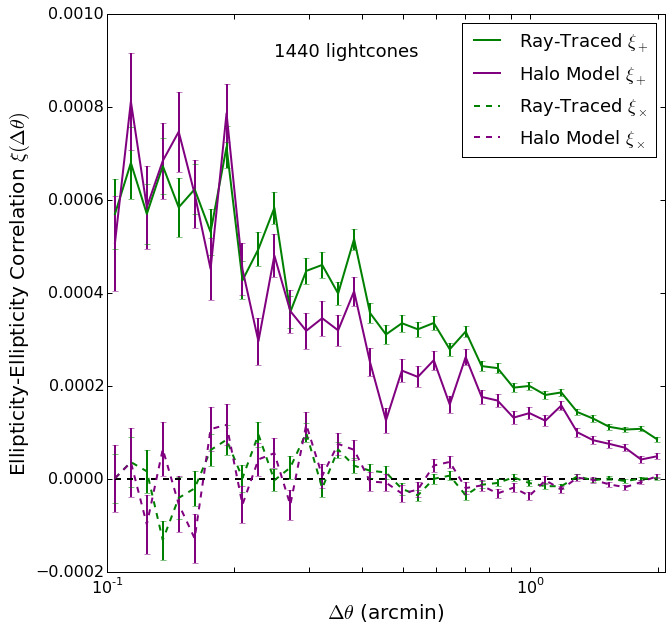
\includegraphics[width=\textwidth]{figs-swe/thesis/gg_corr.png}
        \captionsetup{justification=raggedright,singlelinecheck=false}
        \caption{CAPTION}
        %The ellipticity-ellipticity correlation function for ?? sources at separation distances from 0.1 to 2 arcminutes and a lightcone radius of $R=2$ arcminutes. While the correlation of the intrinsic ellipticities before lensing (blue) shows no correlation, the correlation of the ray-traced ellipticities (green) and halo model predicted ellipticities (purple) both show significant positive correlation on scales up to 1 arcminute. The halo model predicts a small negative correlation above this scale, while the ray-tracing shows positive correlation on all scales.}
        %The correlation of the intrinsic ellipticities before lensing is plotted in blue, and shows no correlation. The correlation of the true ray-traced ellipticities is plotted in green and shows significant positive correlation on all scales. The halo predicted correlation, plotted in purple, shows significant positive correlation until a separation distance of 0.8 arcminutes.
        \label{gg_corr}
    \end{subfigure}
    ~~
    \begin{subfigure}{0.475\textwidth}
        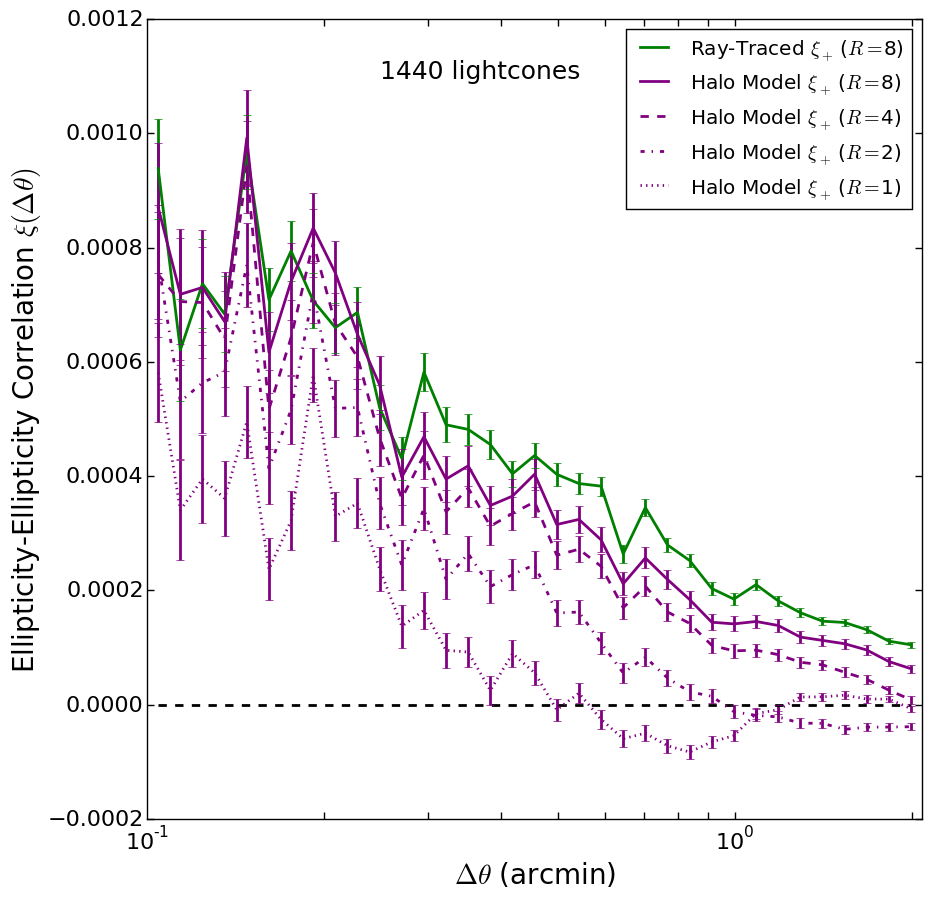
\includegraphics[width=\textwidth]{figs-swe/thesis/gg_progression.png}
        \captionsetup{justification=raggedright,singlelinecheck=false}
        \caption{CAPTION}
        %The ellipticity-ellipticity correlation functions for a series of halo model frameworks with increasing lightcone radii from $R=1$ to $R=8$ arcminutes, all plotted in purple with various line styles. These are compared to the same ray-traced correlation from Figure \ref{gg_corr}.}
        \label{gg_corr_series}
    \end{subfigure}
    \caption{}
\end{figure}
%------------------------------------------------------------------------------------------------------------------------------------------

The first test of the halo model was with the $\varepsilon$-$\varepsilon$ correlation function with a lightcone radius of ?? arcminutes which is given in Figure \ref{gg_corr}. The statistic measured the average correlation between pairs of ellipticities at separation distances between ?? and ?? arcminutes. The cross-component of the correlation function shows no significant deviation from zero as expected, as gravitational lensing only shears galaxies tangentially. For the $\xi_+$ component, the ray-traced (plotted in green) and halo model (plotted in purple) are in relative agreement from seperation scales of ?? to ?? minutes, but there is a clear systematic underprediction of shear power by the halo model on scales larger than ??. This may be indicative that the halo model does not adequately address large-scale mass structures, or that there is significant dark matter mass not correlated with galaxies. The normalized root-mean-square error (NRMSE) of the halo correlation is ??.

Using the same catalog of background sources, this statistic was recalculated for the halo model ellipticities for various lightcone radii ranging from $R_L=1$ to $R_L=8$ arcminutes. The result is shown in Figure \ref{gg_corr_series}, where the series of model predicted correlation functions is compared to the ray-traced correlation function. As $R_L$ increases, the mean number of foreground galaxies contained in each lightcone grows quadratically from ${??\pm??}$ galaxies when $R_L=1$ arcminute to ${??\pm??}$ galaxies when $R_L=8$ arcminutes. Increasing the number of foreground objects, and thus increasing the mass and structure considered for shear and convergence predictions, systematically increased the predicted shear power on all scales. 

%While the series of predicted correlation functions appear to be converging towards the ray-traced correlation function, there is clearly diminishing shear power gains as $R_L$ increases.


%%------------------------------------------------------------------------------------------------------------------------------------------
\subsection{Galaxy-Mass Correlation Function}

The catalog of lensed ellipticities was also analyzed using the galaxy-mass correlation function with separation distances from ?? to ?? arcminutes and a lightcone radius of ?? arcminutes. The result is shown in Figure \ref{ng_corr}. The lensed ellipticities from the ray-tracing and halo model both show positive correlation on all calculated scales and are in agreement on separations from ?? to ?? arcminutes. However, the halo model is still systematically underpredicting the shear power on scales above ?? arcminutes, although now only by an average of ??\%. A new feature is the large overprediction of shear power on separation scales smaller than ?? arcminutes. This is likely because background sources this close to foreground halos are often in the strong lensing regime which is not currently accounted for by the \texttt{Pangloss} framework. The NRMSE of the halo correlation is ??.

The galaxy-mass correlation function was similarly re-calculated at increasing lightcone radii from $R=1$ to $R=8$ arcminutes with the result in Figure ??. As with the $\varepsilon$-$\varepsilon$ correlation, ...

%%------------------------------------------------------------------------------------------------------------------------------------------
%% Galaxy-mass correlation function
\begin{figure}
    \centering
    \begin{subfigure}{0.475\textwidth}
        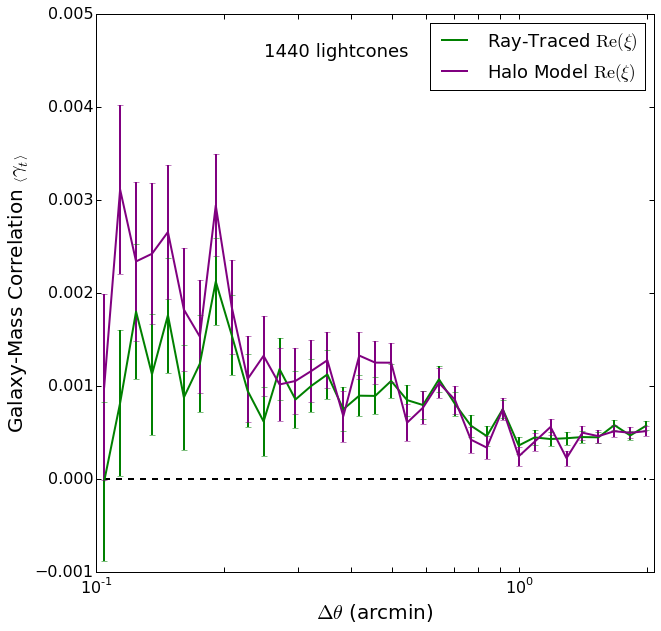
\includegraphics[width=\textwidth]{figs-swe/thesis/ng_corr.png}
        \captionsetup{justification=raggedright,singlelinecheck=false}
        \caption{CAPTION}
        %The galaxy-mass correlation function of 3,240 sources at separation distances from 0.1 to 2 arcminutes and a lightcone radius of $R=2$ arcminutes. There is no significant correlation of the intrinsic ellipticities (blue) as expected, and both the ray-traced correlation (green) and halo model correlation (purple) are positive on all scales. The green and purple curves are in agreement from 0.2 to 0.7 arcminutes, but have significant discrepancies on scales above and below this range.}
        \label{gg_corr}
    \end{subfigure}
    ~~
    \begin{subfigure}{0.475\textwidth}
        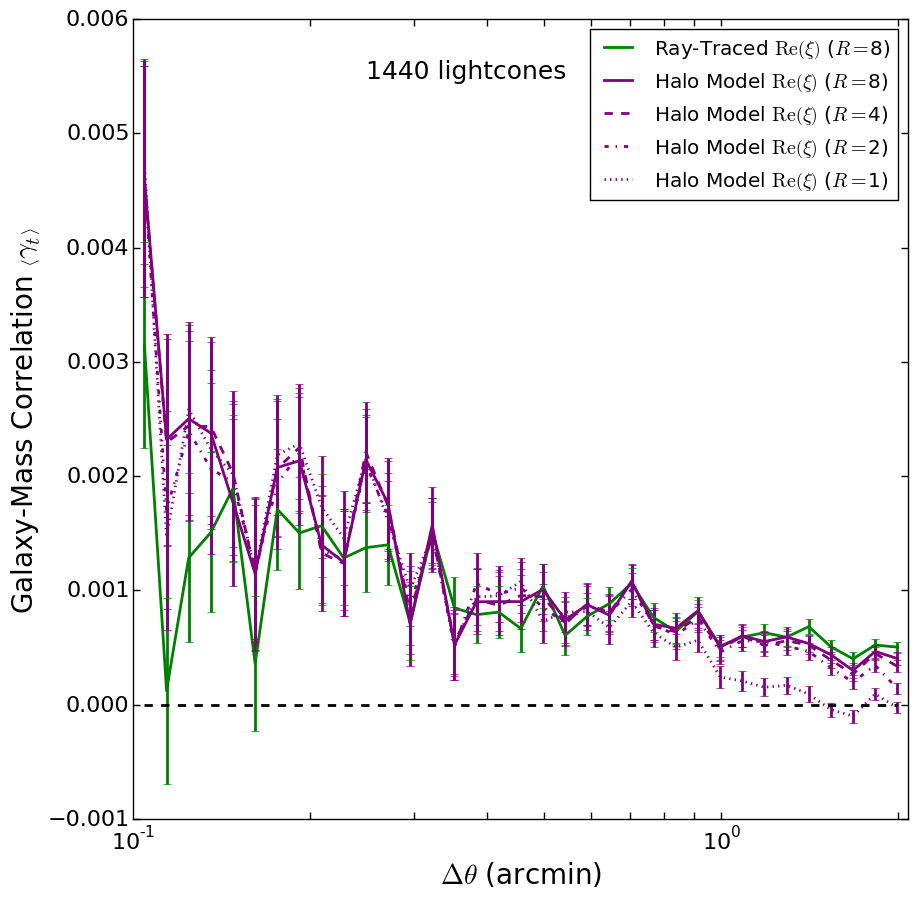
\includegraphics[width=\textwidth]{figs-swe/thesis/ng_progression.png}
        \captionsetup{justification=raggedright,singlelinecheck=false}
        \caption{CAPTION}
        \label{gg_corr_series}
    \end{subfigure}
    \caption{}
\end{figure}
%
%%------------------------------------------------------------------------------------------------------------------------------------------

%%------------------------------------------------------------------------------------------------------------------------------------------
\subsection{Correlation Fraction of Relevant Halos} \label{halo_fraction}

Of intrinsic interest is the relative number of relevant halos needed in each lightcone to accurately predict the halo correlation functions in Figures ?? and ??, as a low percentage would allow much faster lensing predictions. Figure ?? displays an example ellipticity-ellipticity correlation function comparrison of the halo model using all halos (purple) and halo model using halos above the relevance limit of (?? $M_{\odot}/$Mpc$^3$), as well as the percent error of each predicted value between the two implementations. This relevance limit resulted in $??\pm??$ relevant halos per lightcone, and resulted in a normalized root-mean-square error (NRMSE) of ??. Figures ?? plots the ellipticity-ellipticity and galaxy-mass correlation function NRMSE and mean correlation fraction as a function of mean relevant halos. These results suggest that either correlation function prediction can be approximated with an NRMSE below ?? using the ?? most relevant halos. (More analysis after plots have been made)

%%------------------------------------------------------------------------------------------------------------------------------------------
% Correlation Function Comparrison
\begin{figure}
    \centering
    \begin{subfigure}{0.475\textwidth}
        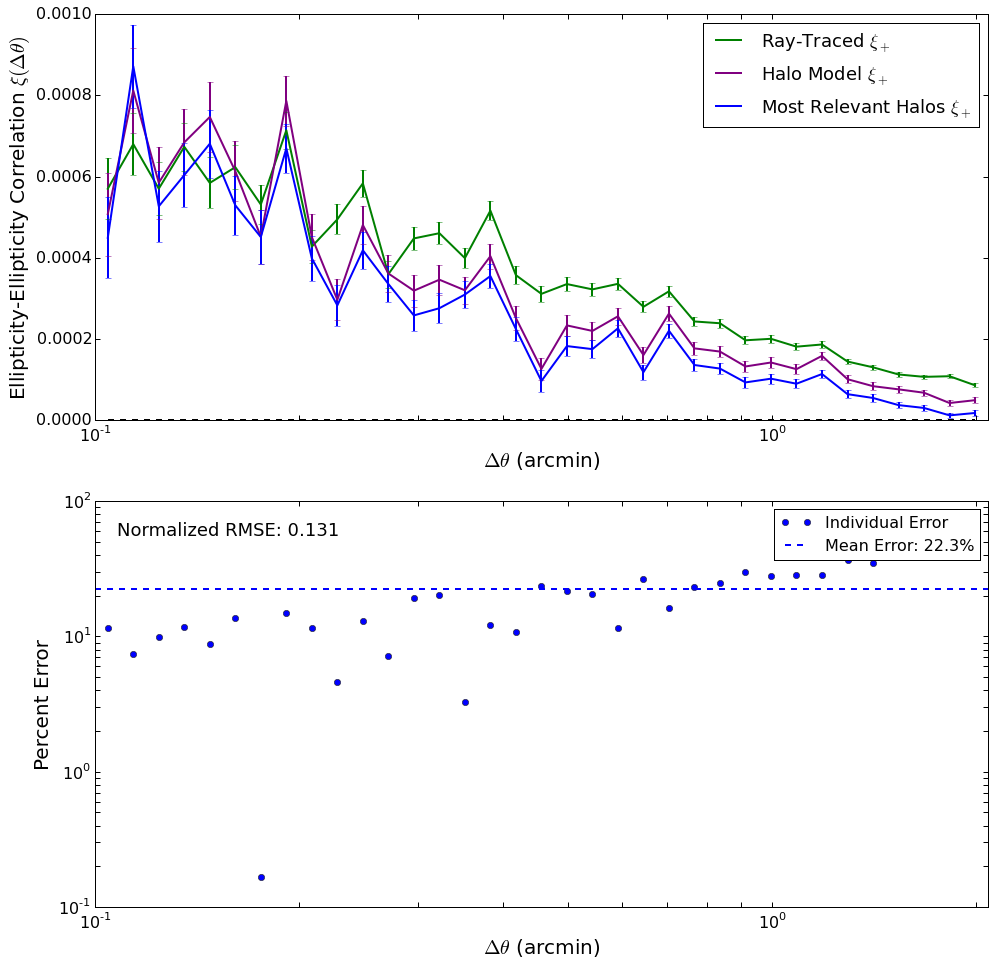
\includegraphics[width=\textwidth]{figs-swe/thesis/rel_gg_compare.png}
        \captionsetup{justification=raggedright,singlelinecheck=false}
        \caption{CAPTION}
        %The ellipticity-ellipticity correlation function for ?? sources at separation distances from 0.1 to 2 arcminutes and a lightcone radius of $R=2$ arcminutes. While the correlation of the intrinsic ellipticities before lensing (blue) shows no correlation, the correlation of the ray-traced ellipticities (green) and halo model predicted ellipticities (purple) both show significant positive correlation on scales up to 1 arcminute. The halo model predicts a small negative correlation above this scale, while the ray-tracing shows positive correlation on all scales.}
        %The correlation of the intrinsic ellipticities before lensing is plotted in blue, and shows no correlation. The correlation of the true ray-traced ellipticities is plotted in green and shows significant positive correlation on all scales. The halo predicted correlation, plotted in purple, shows significant positive correlation until a separation distance of 0.8 arcminutes.
        \label{fig:rel_gg_compare}
    \end{subfigure}
    ~~
    \begin{subfigure}{0.475\textwidth}
        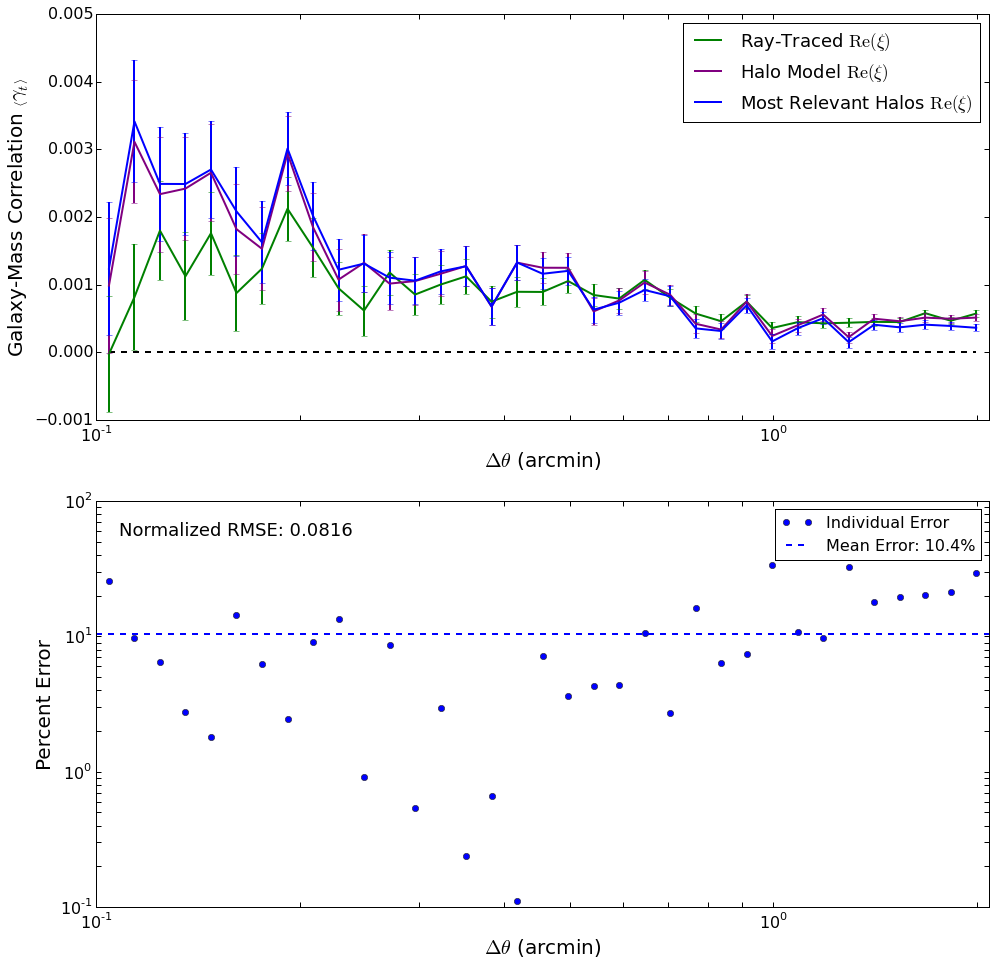
\includegraphics[width=\textwidth]{figs-swe/thesis/rel_ng_compare.png}
        \captionsetup{justification=raggedright,singlelinecheck=false}
        \caption{CAPTION}
        %The ellipticity-ellipticity correlation functions for a series of halo model frameworks with increasing lightcone radii from $R=1$ to $R=8$ arcminutes, all plotted in purple with various line styles. These are compared to the same ray-traced correlation from Figure \ref{gg_corr}.}
        \label{fig:rel_ng_compare}
    \end{subfigure}
    \caption{}
\end{figure}

%------------------------------------------------------------------------------------------------------------------------------------------

%------------------------------------------------------------------------------------------------------------------------------------------
% NRMSE and Correlation Fraction as function of Mean Relevant Halos
% \begin{figure}
%     \centering
%     \includegraphics[width=0.475\textwidth]{figs-swe/thesis/corr_fraction.png}
%     \captionsetup{justification=raggedright,singlelinecheck=false}
%     \caption{CAPTION}
%     \label{corr_fraction}
% \end{figure}

%%------------------------------------------------------------------------------------------------------------------------------------------


%%------------------------------------------------------------------------------------------------------------------------------------------
\subsection{Dark Matter Convergence Mass Maps}

%%------------------------------------------------------------------------------------------------------------------------------------------
%% 3 panel plot of binned Hilbert map, Pangloss map, and difference
\begin{figure*}
    \centering
    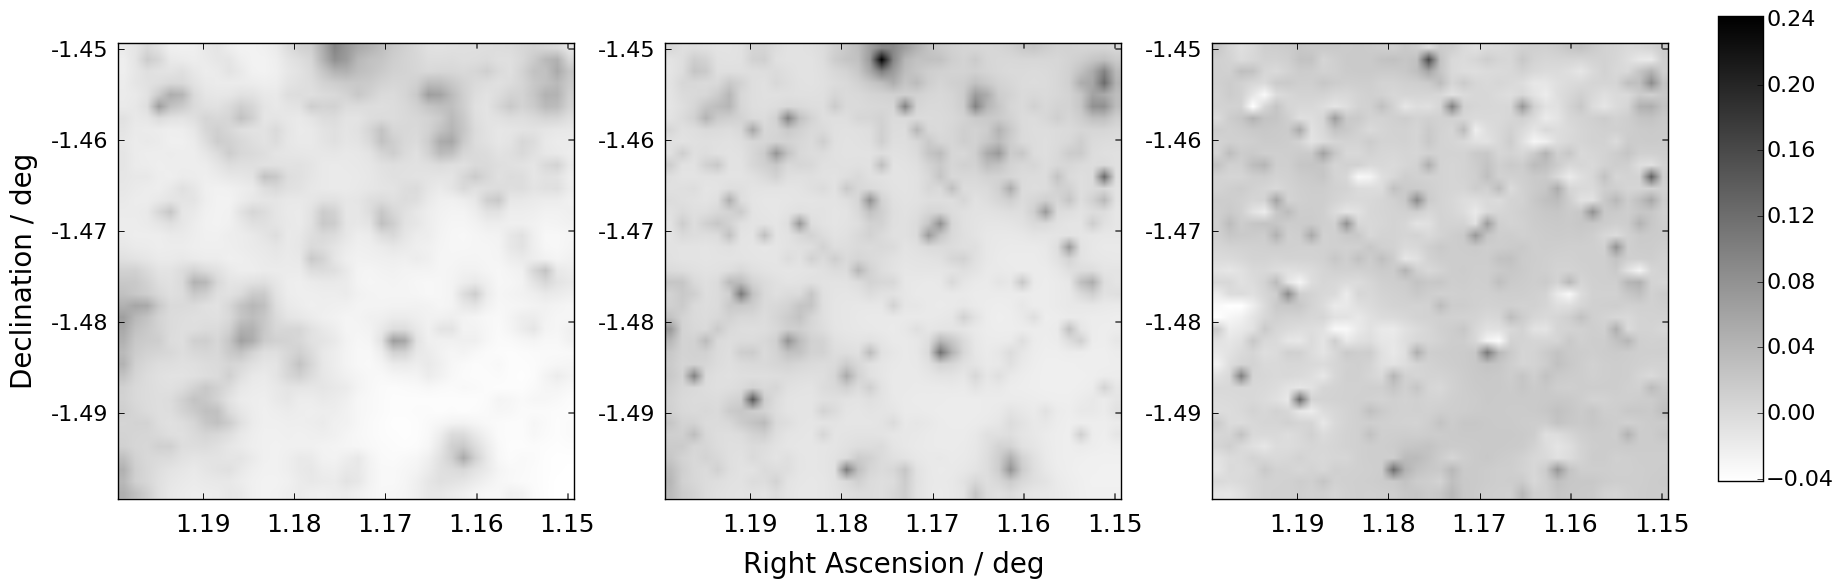
\includegraphics[width=\textwidth]{figs-swe/thesis/kappamaps.png}
    \captionsetup{justification=raggedright,singlelinecheck=false}
    \caption{CAPTION}
    \label{fig:kappamaps}
\end{figure*}
%
%%------------------------------------------------------------------------------------------------------------------------------------------

While correlation functions can describe how well the lensing predictions are being made globally, it is still instructive to analyze the difference between the ray-traced and halo model projected mass maps. This was done by selecting a region of foreground mass, calculating the ray-traced and \texttt{Pangloss}-predicted convergence of a uniform grid of background sources in the field, and binning the convergence maps to a desired resolution. Convergence is proportional to projected surface mass density, so comparring the two convergence maps is equivalent to comparing their respecitve projected mass distributions.

The result of a particular ?? arcmin$^2$ field is shown in Figure \ref{fig:kappamaps}, where the ray-traced convergence is shown on the left, the halo model convergence is in the center, and the ray-traced convergence subtracted from the halo model convergence is shown on the right. While particular foreground masses are almost always predicted, the currently implemented halo model over-predicts the convergence throughout most of the field. The halo model does not appear to accurately account for the voids between foreground masses and over-predicts the mass of most ... This could partially be a result of incorrect halo profiles, but it is apparent that the smooth-component correction is not adequate to ...

%%------------------------------------------------------------------------------------------------------------------------------------------
\subsection{Computational Performance}

A secondary goal of this research was to investigate how quickly the prediction for the shear and convergence for a single background source could be made. The mean CPU time required for the prediction per lightcone was ${??\pm??}$ ms for the first run. However, many small improvements to the coding infrastructure of \texttt{Pangloss} were made to speed up the prediction. The average CPU time for a lensing prediction per lightcone for four separate runs after various (and cumulative) changes is plotted in Figure \ref{cpu_plot}, with a final run time of $??\pm?$ ms. Run 1 corresponds to the original \texttt{Pangloss} framework code, run 2 only wrote the needed quantities for this analysis to the catalog \texttt{Astropy} tables, run 3 changed the redshift grid binning to be done once for all halos in the drilling rather than for every individual halo in lensing, run 4 optimized various lensing calculations with matrices whenever possible, run 5 replaced the computationally expensive lensing calculation functions with a lookup table, and run 6 is using only the most ?? relevant halos. Cumulatively, these changes alone accounted for a ??\% decrease in mean CPU time per lightcone and ?? the initial variation.

%%------------------------------------------------------------------------------------------------------------------------------------------
% Mean lightcone CPU time
\begin{figure}
    \centering
    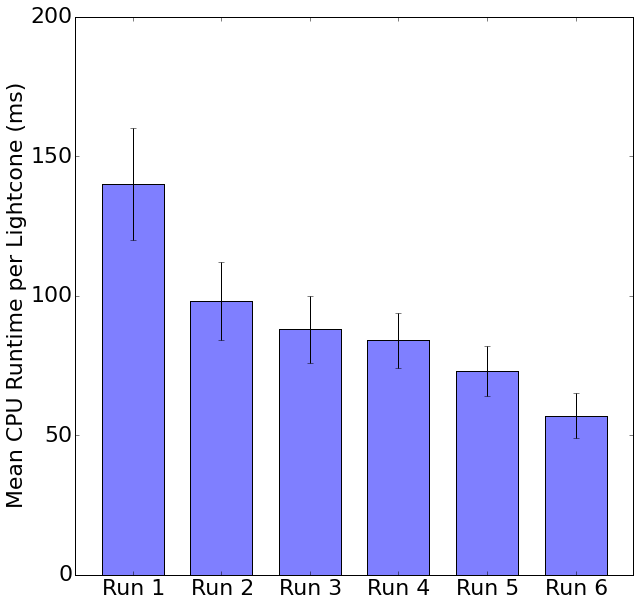
\includegraphics[width=0.475\textwidth]{figs-swe/thesis/profile_bar.png}
    \captionsetup{justification=raggedright,singlelinecheck=false}
    \caption{OLD: The mean CPU runtime per lightcone for various runs with different (and cumulative) code optimizations described in the text. The cumulative changes account for a ??\% decrease in the mean CPU time and a ?? of the variation. Currently, the prediction can be made for a single lightcone in\\$??\pm??$ ms.}
    \label{fig:cpu_plot}
\end{figure}
%%------------------------------------------------------------------------------------------------------------------------------------------

%%==========================================================================================================================================
\section{Feasibility of Parameter Inference using Pangloss} \label{feasibility}

One of the long-term goals of \texttt{Pangloss} is to be able to use all available sky survey data (sky positions, stellar masses, magnitude, photometric redshift, ellipticities, etc.) to make a hierarchial inference of the Universe's cosmological and galaxy population model hyper-parameters such as the density paramters $\Omega_m$ and $\Omega_\Lambda$, the Hubble constant $H_0$, and stellar mass-halo mass relation \cite{smhr}. This is a large undertaking and will require considerable testing and calibration on large N-body simulations such as the Millennium Simulation. As a first step towards this goal, I attempted to gague the feasibility of implementing two methods of parameter inference, maximum likelihood estimation and approximate Bayesian computation, using the current framework. The results of this feasibility test, particularly the CPU time per likelihood estimation, will help guide fugure work on \texttt{Pangloss}. For a detailed description of a probablistic modeling approach to gravitational lensing inference for large sky surveys, see \cite{grav_lens_inference}. Exploratory notes of implementing such an inference in the framework is available on \texttt{Pangloss}'s public github repository\footnote{https://github.com/drphilmarshall/Pangloss/issues/23}.\\

(Introduce Bayes' Theorem, likelihood, prior, posterior, etc.??)


%%------------------------------------------------------------------------------------------------------------------------------------------
\subsection{Likelihood Estimation} \label{mle}

Perhaps the most common method of parameter estimation of statistical models is called maximum-likelihood estimation (MLE). The likelihood is a function of the parameters of a statistical model that measures the probability of a data set or outcomes given the model parameters \cite{??}. It is the mathematical answer to the question, ``\textit{Given a particular set of parameters, what is the probability that this data set could have occured?}" The form of the likelihood depends on the properties and circumstances of the data but generally has the form of the product of the probability density function $f$ of each individual observation $x_i$ given model parameters $\vec{\theta}$ \cite{likelihood}:
\begin{equation}
\mathcal{L}(\vec{\theta},x_1,x_2,\ldots,x_n)=\prod_{i=1}^nf(x_i|\vec{\theta}).
\end{equation}

A much more detailed introduction to likelihood and MLE is given in \cite{likelihood}. For this work, the likelihood is given by \cite{marshall_thesis}:
\begin{equation}\label{likelihood}
\mathcal{L}(\Sigma|\varepsilon_{i,j},g_{i,j})=\frac{1}{Z_L}\exp\left(\frac{-\chi^2}{2}\right),
\end{equation}

\noindent where $\varepsilon_i,j$ is the $j$-component of the $i$-th predicted lensed galaxy ellipticity, $g_i,j$ is the $j$-th component of the `true' reduced shear corresponding to $\varepsilon_i$, $\chi^2$ is the typical test statistic
\begin{equation}\label{chi2}
\chi^2=\sum_{i=1}^N\sum_{j=1}^2\frac{(\varepsilon_{i,j}-g_{i,j})^2}{\sigma^2},
\end{equation}

\noindent the normalization factor $Z_L$ is
\begin{equation}
Z_L=(2\pi\sigma^2)^{(2N)/2},
\end{equation}

\noindent where $N$ is the number of background galaxies (the $2N$ exponent is a result of the two ellipticity components for each of the $N$ galaxies), and the uncertainty in galaxy ellipticity estimation $\sigma$ is the sum in quadrature of the dispersions of intrinsic and `observed' (i.e. \texttt{Pangloss}-predicted) ellipticities:
\begin{equation}\label{sigma}
\sigma=\sqrt{\sigma_{\text{int}}^2+\sigma_{\text{obs}}^2}.
\end{equation}

While this works in principle, computationally it is much easier to work with the natural logarithm of the likelihood function called the log-likelihood. As the logarithm is a monotonically increasing function, the likelihood and log-likelihood achieve their maximum at the same points and so can be used interchangably in maximum likelihood estimation. From Equations \eqref{likelihood}-\eqref{sigma} is follows that the log-likelihood is given by
\begin{align}\label{log-likelihood}
\ln\mathcal{L}&=-\ln Z_L-\frac{1}{2}\chi^2\nonumber \\
&=-\frac{N}{2}\ln(2\pi\sigma)-\frac{1}{2}\sum_{i=1}^N\sum_{j=1}^2\frac{(\varepsilon_{i,j}-g_{i,j})^2}{\sigma^2}.
\end{align}

To use \texttt{Pangloss} to infer hyperparameters using MLE, a set of trial parameters would be sampled from appropriate prior distributions and used to calculate the lensed ellipticities of a mock background catalog using the methodology shown in Section \ref{pangloss}. The log-likelihood of this set of parameters would be calculated using Equation \eqref{log-likelihood}, and the process would be repeated for many parameter combinations until a sufficient approximation of the likelihood is made. The most likely hyperparameters would then simply be the set of parameters that led to the maximum likelihood.

However, exploring the parameter space efficiently is a significant problem in MLE, especially in a dataset such as this which there are potentially millions or even billions of parameters (i.e. halo masses). For this thesis, I only compute the log-likelihood for a small handful of parameter sets to gague how feasible such an inference would be in future work with far more computational power.

%%------------------------------------------------------------------------------------------------------------------------------------------
\subsection{Approximate Bayesian Computation} \label{abc}

MLE is not the only common method of parameter inference. As discussed in the previous section, the likelihood is computationally expensive to calculate and so MLE may not lend itself well to inference when large number of background galaxies are used. Approximate Bayesian computation (ABC) is a class of computational methods that estimate the posterior distribution without calculating the likelihood function. This can be vital for complex models in which the likelihood function does not have an analytic form or is computationally costly to evaluate. While fortunately Equation \eqref{log-likelihood} is a relatively simple likelihood function, the calculation may become too costly for very large mock catalogs of millions or billions of source galaxies. However, ABC does come at a cost; as the name implies, there are various assumptions and approximations made in the process that can potentially lead to an innaccurate posterior prediction. A general overview of the ABC process is shown in Figure \ref{fig:abc} taken from (first author name et al.) \cite{abc}, which offers an excellent introduction to the topic. I summarize a common ABC implementation and its application to \texttt{Pangloss} below.

% In order to gague future inference feasibility, I analyzed whether ABC could make posterior 

All ABC methods approximate the likelihood function by simulating data using parameters sampled from the prior distribution. If the simulated data are very `similar' to the observed data, then the parameter set is accepted; if not, the parameter set is rejected. The posterior is then approximated by a histogram of the accepted parameters after a large number of simulations have been run. These methods are approximations as simulated data that is `similar enough' to observed data is accepted rather than requiring exact matches. Practically, determining what metric of `similar' to use and what threshold value $\delta$ should be chosen for data rejection becomes a compromise of computation speed and posterior accuracy.

ABC using a simple distance metric like Euclidean distance or $\chi^2$ is highly inefficient for data with large dimensionality as the probability of the `distance' being small quickly vanishes. Instead, the similarity of observed and simulated data is often characterized by summary statistics such as mean and variance for simple data or correlation functions for more ... data. Thus an ABC rejection algorithm reduces to predicting the summary statistic for the simulated data, comparing to the corresponding summary statistic of the observed data, and basing rejection on a chosen threshold of difference in summary statistics.

A possible implemenetation of the above for \texttt{Pangloss} would be as follows: Choose the the ray-traced lensed ellipticities as the `observed' data and compute its $\varepsilon$-$\varepsilon$ correlation function to be used as the desired summary statistic. Let the distance metric to be the NRMSE between the predicted and ray-traced $\varepsilon$-$\varepsilon$ correlation function. Compute the best-case $\varepsilon$-$\varepsilon$ correlation function using all halo data as shown in Section \ref{pangloss} and make the threshold value $\delta$ be some multiple of the best-case NRMSE (e.g. ${\delta=2\cdot\text{RMSE}_{\text{best-case}}}$. Create mock data by repeating the methodology in \ref{pangloss} except use the stellar mass-halo mass relation, dependent on paramters we sample from a prior, to predict halo masses based upon each galaxy's stellar mass. Compute the simulated $\varepsilon$-$\varepsilon$ correlation function and determine whether to accept or reject the data by determining if the NRMSE is below the threshold $\delta$. The posterior will be estimated after a large number of iterations through the rejection algorithm.

%%------------------------------------------------------------------------------------------------------------------------------------------
% ABC Diagram
\begin{figure}
    \centering
    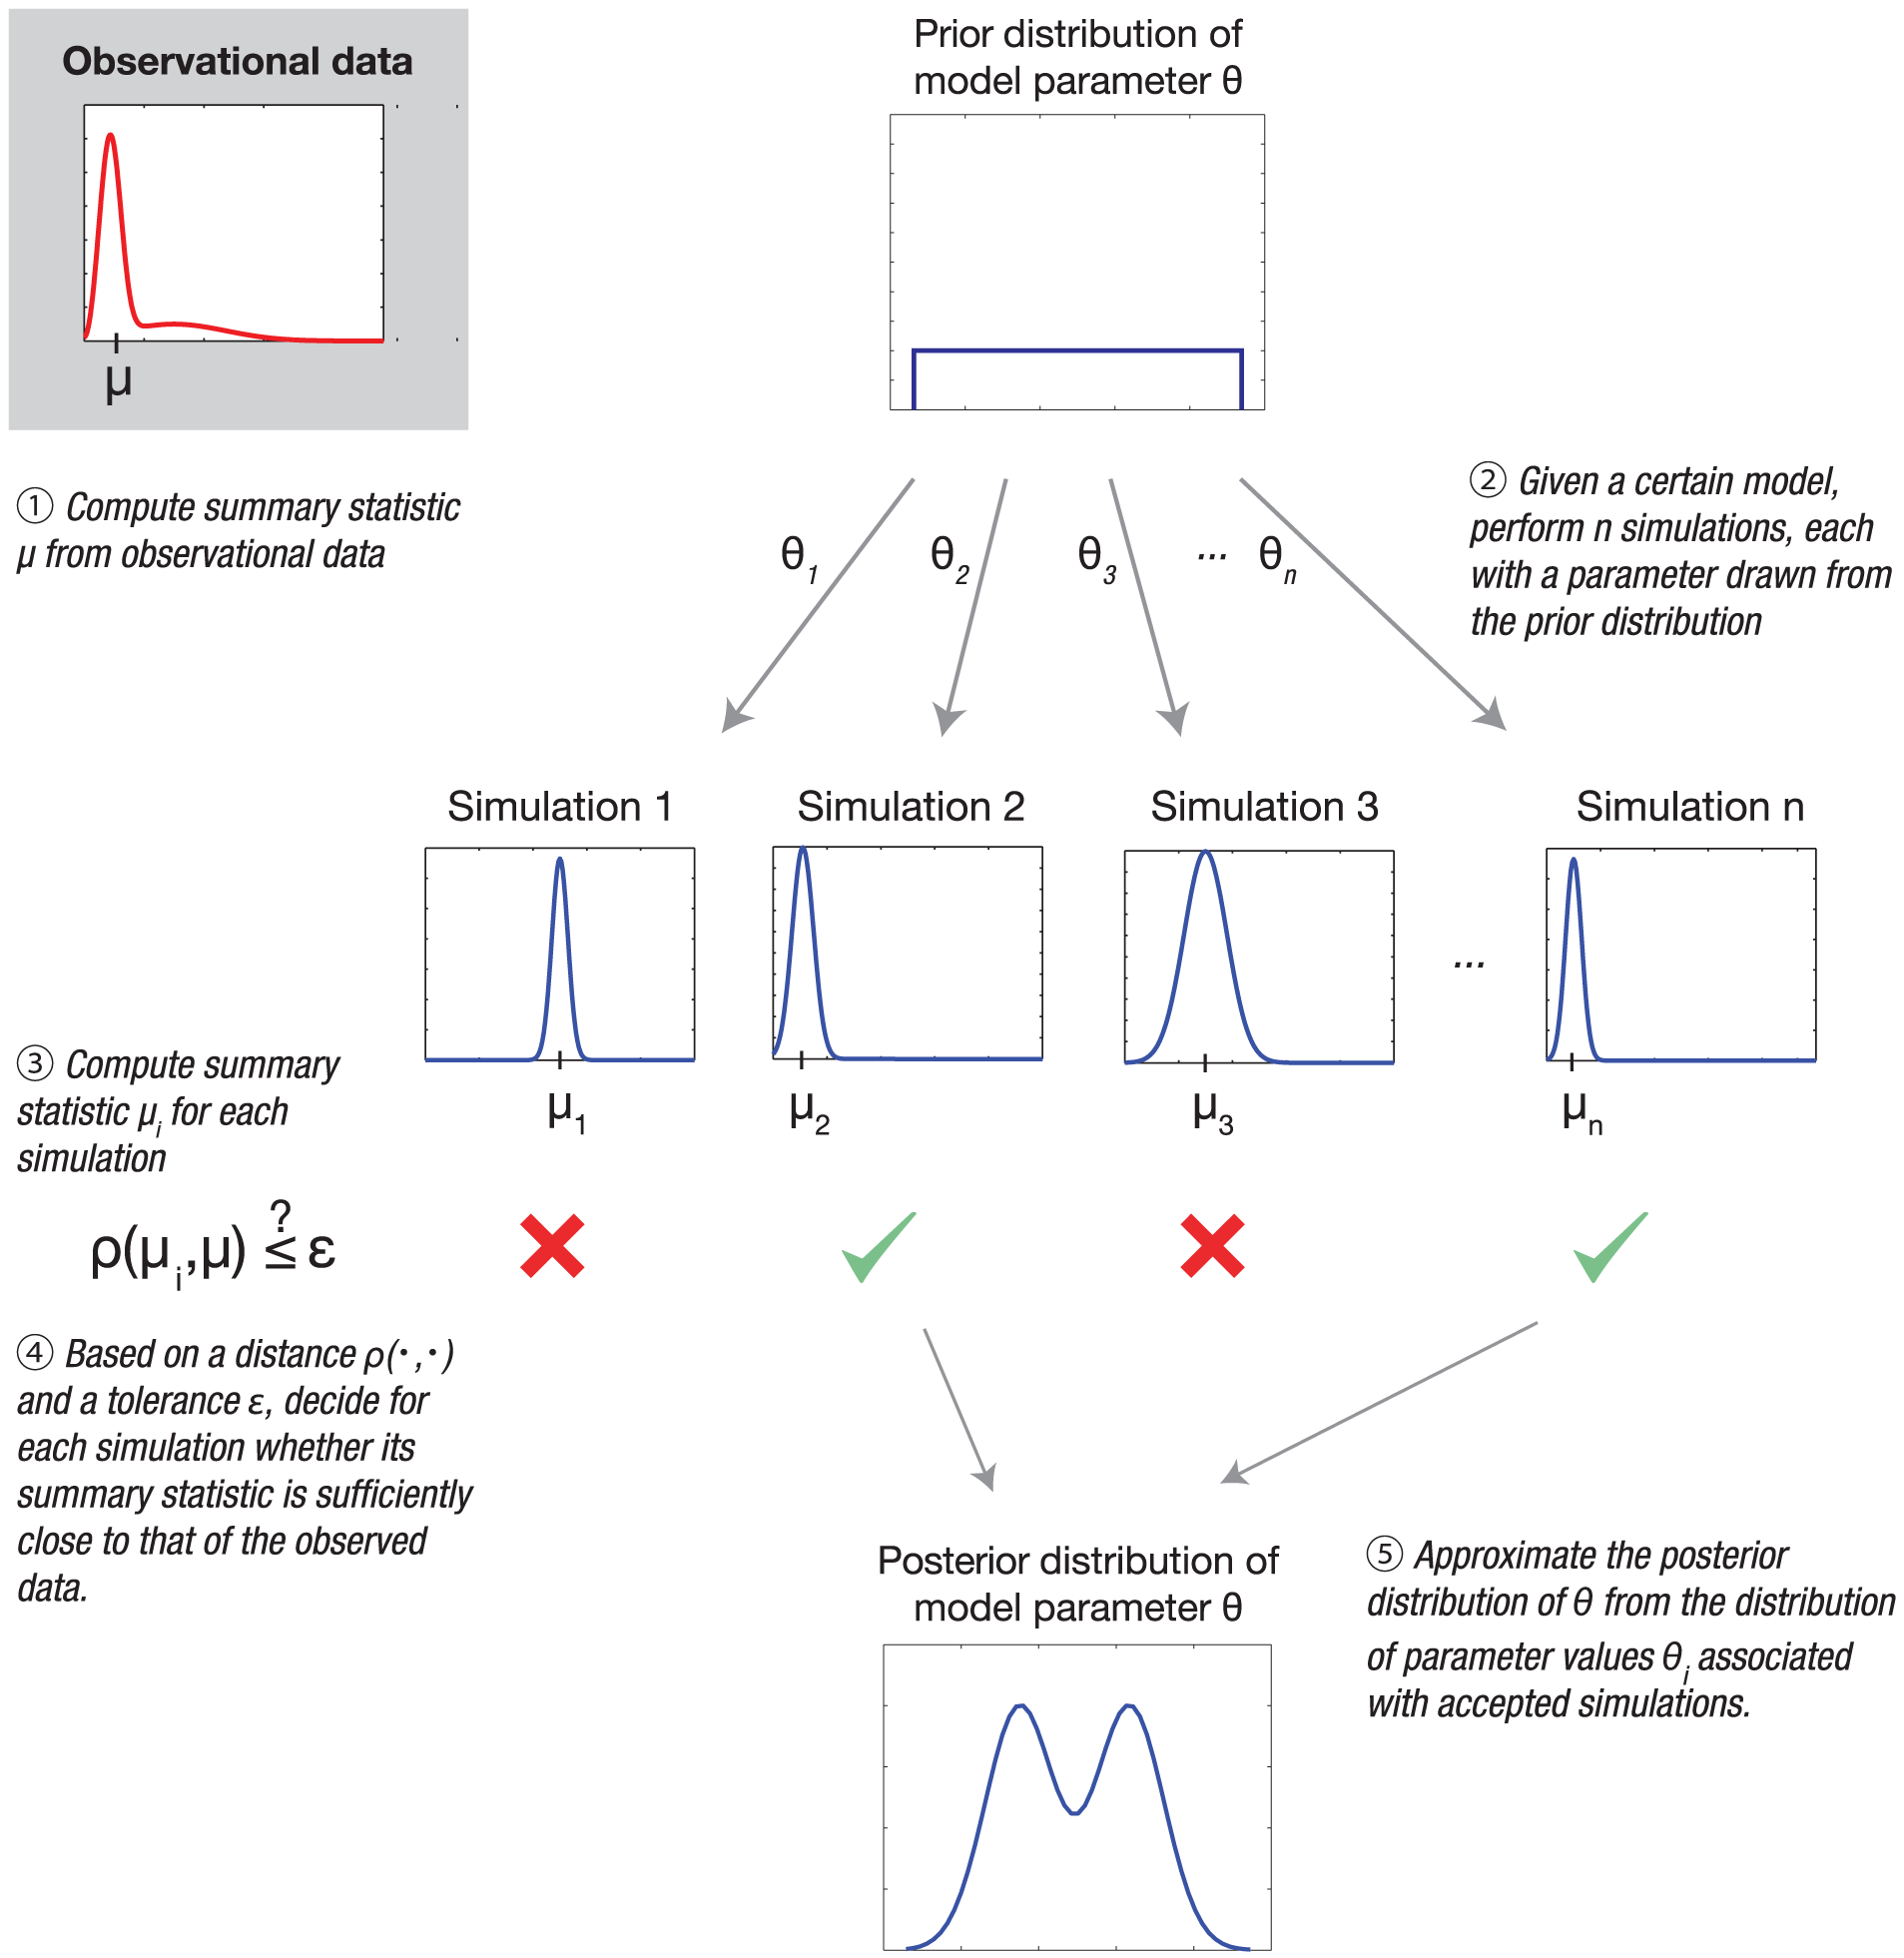
\includegraphics[width=0.5\textwidth]{figs-swe/thesis/abc.png}
    \captionsetup{justification=raggedright,singlelinecheck=false}
    \caption{CAPTION; Will replace with a self-made plot made specifically for \texttt{Pangloss} before thesis submission.}
    \label{fig:abc}
\end{figure}
%%------------------------------------------------------------------------------------------------------------------------------------------

%%------------------------------------------------------------------------------------------------------------------------------------------
\subsection{Results}

I implemented the methodology in section \ref{Pangloss} to make weakly lensed ellipticity predictions in 10 mock catalogs of $N$ background sources ranging from $N=??$ to $N=??$. The mean CPU times for a single likelihood calulation and ABC rejection decision as a function of $N$ is shown in Figure \ref{mle_vs_abc}. (Clearly abc is slower, and inherently approximate, and requires arbitrary threshold cutoff, so clearly we will be using MLE moving forward.) Additionally, the time spent for either inference method is quite small; the CPU time per likelihood estimation or ABC rejection decision are \textit{far} less than the CPU time required to create lightcones and make the LOS lensing prediction. This is an encouraging result and suggests that further work on the framework should be on additional optimization of the lensing prediction code rather than posterior estimation.


%%------------------------------------------------------------------------------------------------------------------------------------------
% ABC Diagram
% \begin{figure}
%     \centering
%     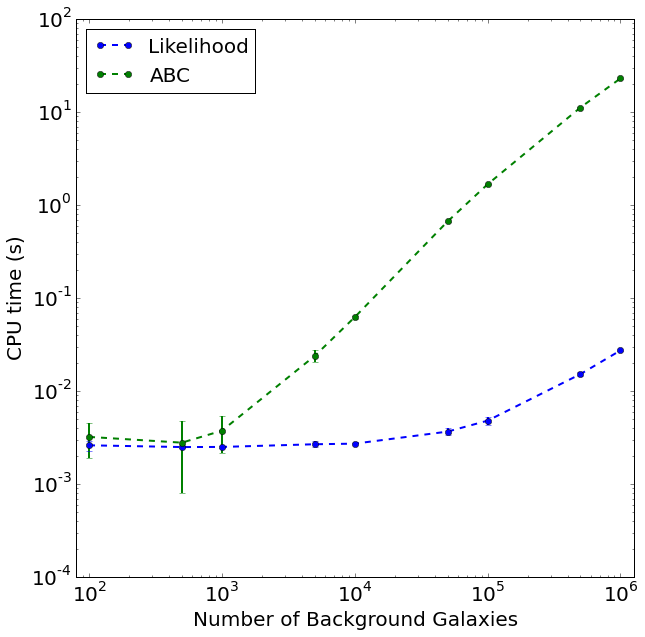
\includegraphics[width=0.475\textwidth]{figs-swe/thesis/mle_vs_abc.png}
%     \captionsetup{justification=raggedright,singlelinecheck=false}
%     \caption{CAPTION}
%     \label{fig:mle_vs_abc}
% \end{figure}
%%------------------------------------------------------------------------------------------------------------------------------------------

%%==========================================================================================================================================
\section{Discussion}


%%------------------------------------------------------------------------------------------------------------------------------------------
\subsection{Issues with the Halo Model}

\begin{enumerate}
\item Under-predicting shear on large scales
\item Not accounting for strong lensing
\item Smooth-component correction not enough
\end{enumerate}

% OLD: Both the ellipticity-ellipticity and galaxy-mass correlation functions show clear issues with using the halo model to predict the lensing of background sources with \texttt{Pangloss}, even in the best-case scenario of perfect knowledge of the halo masses and their spectroscopic redshifts. The systematic underprediction of shear power present in both correlation functions is likely do to missing features in the model such as clusters, filaments, and voids.

% While individual galaxies currently receive halos, a cluster of galaxies will sit in an larger halo whose presence is not being considered as its position, mass, and extent are difficult to determine. The absence of this mass undoubtedly effects shear predictions and ellipticity correlations on large scales. While some of the filament structure is captured in the framework, as the higher density of galaxies in filaments will lead to a higher density of halos, any additional dark matter structure between halos and clusters is not being accounted for. While difficult to do in practice, one can imagine connecting clusters of galaxies with dark matter `cylinders' to account for the extra filament mass. Voids are also not currently considered, as the framework assumes the field has constant mass density equal to that of the average mass density of the universe and then adds halo masses on top of this density. This would make the average matter density across the field \textit{larger} than the mean density of the universe, and could be counteracted by subtracting mass from regions in between foreground halos. Stellar masses could also be incorporated into the \texttt{Pangloss} prediction, but any effect would likely be dominated by the missing features described above.

% The progression of model predicted ellipticity-ellipticity correlation functions at larger radii converging to the ray-traced correlation in Figure \ref{gg_corr_series} supports the analysis given above, as the prediction was progressively better with larger number of foreground halos and thus more mass and structure. However, the number of foreground objects scales quadratically with the lightcone radius making it prohibitively expensive above $R=8$ arcminutes. With a radius this large, most foreground objects will be too far away from the line of sight and have insufficient mass to make a significant contribution to the lensing of the background source. This suggests the creation of a metric to predict the `relevance' of each halo to the lensing contribution. In this way, the framework could be restructured to only use the most important halos in the computationally expensive lensing prediction, while simultaneously allowing for larger lightcones with more relevant halos. This could aid in the aforementioned shear power prediction issues.



%%------------------------------------------------------------------------------------------------------------------------------------------
\subsection{Most Halos are not Relevant}

From Section \ref{halo_fraction}, we clearly do not need to use all halos in the field to predict the best-case scenario correlation functions within a mean ??\% error or NRMSE below ??. (more).


%%------------------------------------------------------------------------------------------------------------------------------------------
\subsection{Scaling Up Pangloss}

While the current \texttt{Pangloss} framework can handle the lensing predictions of ?? sources in a ?? arcmin$^2$ field comfortably on a single processor, the goal is to scale up the framework to make predictions for background sources of the same number density in a 100 deg$^2$ field; this will require 3.6 million lightcones, each containing at least ??? relevant foreground halos. Luckily, the prediction is trivially parallelizable as the shear and convergence calculation of each lightcone is independent of all other lightcones. This makes GPUs an attractive candidate for future work, as it would only take 360 GPUs with 10,000 threads each to carry out the prediction. Additionally, the ?? MB of RAM per lightcone is sufficiently small to fit 10,000 lightcones on a GPU.\\

(More??)


%%------------------------------------------------------------------------------------------------------------------------------------------
\subsection{Future Inference Work}

The results of Section \ref{feasibility} demonstrated that the likelihood calculation does not present a computational issue in comparrison to the lensing calculation, so MLE is a feasible approach for a hierarchial inference of the stellar mass-halo mass relation. A single ABC rejection algorithm in fact performed \textit{worse} than a single likelihood calculation, so clearly ABC is not suitable for this work. However as discussed above, there is still much more work to the \texttt{Pangloss} framework that needs to be done, both in modeling features and computational infastructure, before an inference using a large number of background sources comparable to modern sky surves can be achieved.


%%==========================================================================================================================================
\section{Conclusion}

% OLD: In this paper, a simple halo model was used to reconstruct all the mass along lines of sight in the Millennium Simulation to make predictions of how foreground mass weakly lensed the ellipticities of 3,240 generated background sources across a field of 324 arcmin$^2$. The lensed ellipticities were characterized globally using the ellipticity-ellipticity and galaxy-mass correlation functions and then compared with the same statistics from ray-traced data. There was a systematic-underprediction of shear power on all scales in the ellipticity-ellipticity correlation function as well as an absence of any predicted correlation on scales larger than 1 arcminute, suggesting missing features in the \texttt{Pangloss} framework. The galaxy-mass correlation function predicted by the halo model was in agreement with the ray-traced correlation function on scales from 0.2 to 0.7 arcminutes, but significantly overpredicted the shear power on smaller scales due to strong lensing effects. Now that a proof of concept has been demonstrated, there is work being done to scale up the \texttt{Pangloss} framework to make lensing predictions over 100 deg$^2$ using far more computational resources. While the results are encouraging for such a simple model, many strong and unrealistic assumptions were made in the methodology that limit its use in observational surveys. In the future, a similar analysis should be made after relaxing some of the assumptions to see how different the predictions by the halo model are from this best-case scenario.


%%==========================================================================================================================================
\section{Acknowledgements}

% OLD: I would like to thank the Department of Energy for funding this research and giving me this wonderful opportunity, as well as SLAC National Laboratory for hosting me. 

%This work was greatly aided by numerous conversations with Risa Wechsler from Stanford University and Matt Becker from the Kavli Institute for Particle Astrophysics and Cosmology (KIPAC), as well as Jesus Pando from DePaul University. Finally, I am incredibly grateful to Phil Marshall for his unending support, patience, and guidance throughout this research.
% This work was supported in part by the U.S. Department of Energy, Office of Science, Office of Workforce Development for Teachers and Scientists (WDTS) under the Science Undergraduate Laboratory Internships Program (SULI).

%%==========================================================================================================================================

\onecolumngrid

\vspace{0.25 in}

\section{References}
\vspace{-.2825in}
\bibliographystyle{unsrt}
\bibliography{suli-report-swe}


%%==========================================================================================================================================

\newpage

\section{Appendix}

%%------------------------------------------------------------------------------------------------------------------------------------------
\subsection{Visualizing Correlation Functions}

%% Correlation Colormaps
\begin{figure}[!b]
    \centering
    \begin{subfigure}{0.425\textwidth}
        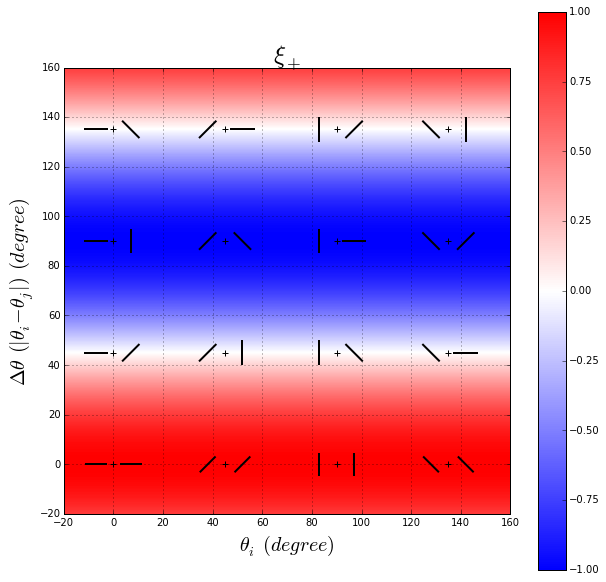
\includegraphics[width=\textwidth]{figs-swe/xip_colormap.png}
        \captionsetup{justification=raggedright,singlelinecheck=false}
        \caption{The positive tangential component of the $\varepsilon$-$\varepsilon$ correlation as a function of galaxy orientation plotted as a colormap. The correlation component is positive for parallel galaxies, negative for perpendicular galaxies, and zero for galaxies offset by 45$^\circ$.}
        \label{xip_colormap}
    \end{subfigure}
    ~
    \begin{subfigure}{0.425\textwidth}
        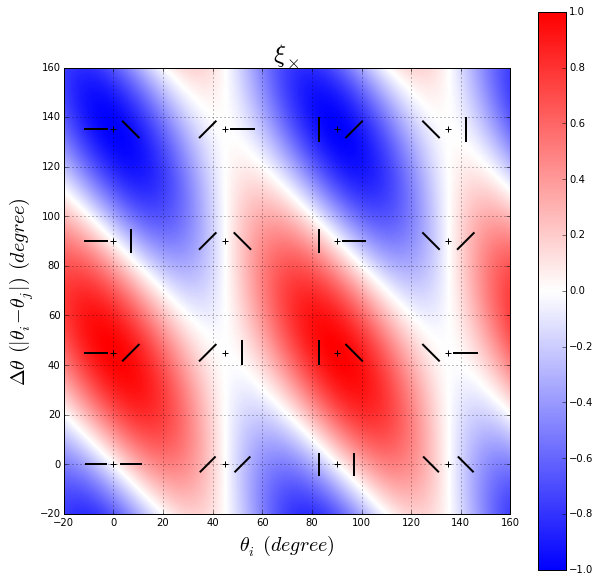
\includegraphics[width=\textwidth]{figs-swe/xix_colormap.png}
        \captionsetup{justification=raggedright,singlelinecheck=false}
        \caption{The cross component of the $\varepsilon$-$\varepsilon$ correlation as a function of galaxy orientation plotted as a colormap. While the pattern is more complicated than that of the tangential component, note that the correlation is zero for all preferred orientations after lensing.}
        \label{xix_colormap}
    \end{subfigure}
    \caption{Correlation pair colormaps for $\xi_+$ and $\xi_\times$.}
    \label{corr_colormaps}
\end{figure}

(Might need to rework some phrasing)\\

At first encounter, the use of correlation functions to analyze data can be difficult to comprehend, let alone visualize. While by no means a thorough or mathematical analysis (see \cite{correlation_functions} for a more formal introduction), I have created some explanatory plots to aid in visualizing how weakly lensed ellipticities can be measured with correlation functions and place the main results of this paper in more context.

The main statistic used in this work is the ellipticity-ellipticity ($\varepsilon$-$\varepsilon$) correlation function, which has two tangential components $\xi_\pm$ and a cross component $\xi_\times$. The components most interesting for gravitational lensing are the positive tangential component $\xi_+$, expected to be positive for lensed galaxies, and the cross component $\xi_\times$, which is expected to be zero. To get an intuition for what these quantities measure, first consider the correlation values for individual pairs of galaxies as shown in Figure \ref{corr_colormaps}. In each plot, the value of the correlation between two galaxies as a function of their relative orientation is plotted as a colormap with a few sampled galaxy orientations superimposed. For $\xi_+$ the correlation is positive for parallel galaxies, negative for perpendicular galaxies, and zero for galaxies offset by 45$^\circ$. In contrast, $\xi_\times$ is zero for all parallel and perpendicular orientations while nonzero for most 45$^\circ$ offsets. As gravitational lensing shears source images tangentially around a foreground mass, the tangential component is a measure of how similarly two galaxies are lensed, while the cross component is an estimate of the bias (as it should be zero).

Now consider a region of space around a foreground lens populated with many background sources \textit{before lensing}, as in Figure \ref{color_corr_unlensed}. In this plot, source ellipticities are plotted as sticks and colored by their distance from the lens. Calculating the $\xi_+$ component correlation pairs for all galaxies in the same color bin and making a scatter plot as a function of the separation distance between the source pairs, we find the distribution in Figure \ref{corr_dist_unlensed}. The $\xi_+$ component of the $\varepsilon$-$\varepsilon$ correlation function is simply the average of this scatter plot binned in separation distances along the $x$-axis. As the scatter is randomly distributed around zero, the $\varepsilon$-$\varepsilon$ correlation function for un-lensed sources should be zero on all scales.

%% Color-Coded Correlation Un-lensed
\begin{figure}
    \centering
    \begin{subfigure}{0.45\textwidth}
        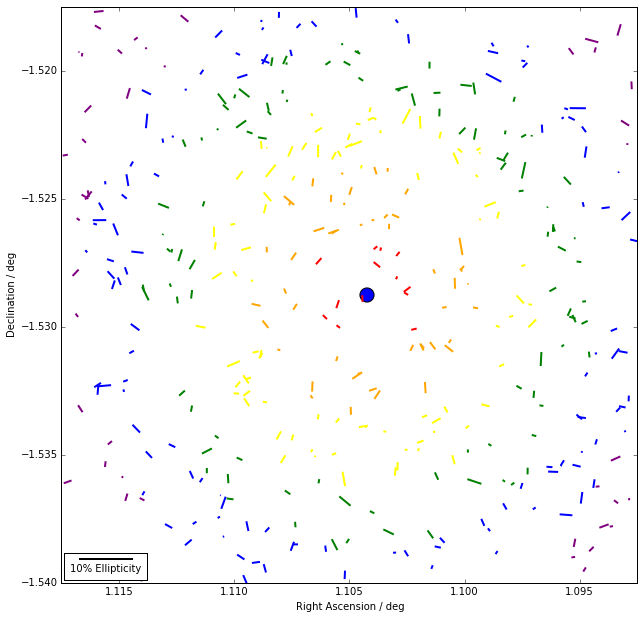
\includegraphics[width=\textwidth]{figs-swe/corr_visualization_unlensed.png}
        \captionsetup{justification=raggedright,singlelinecheck=false}
        \caption{A set of background sources around a foreground lens (blue dot). The size and orientation of each stick represents the intrinsic source ellipticity and is colored by the distance away from the lens.}
        \label{color_corr_unlensed}
    \end{subfigure}
    ~
    \begin{subfigure}{0.45\textwidth}
        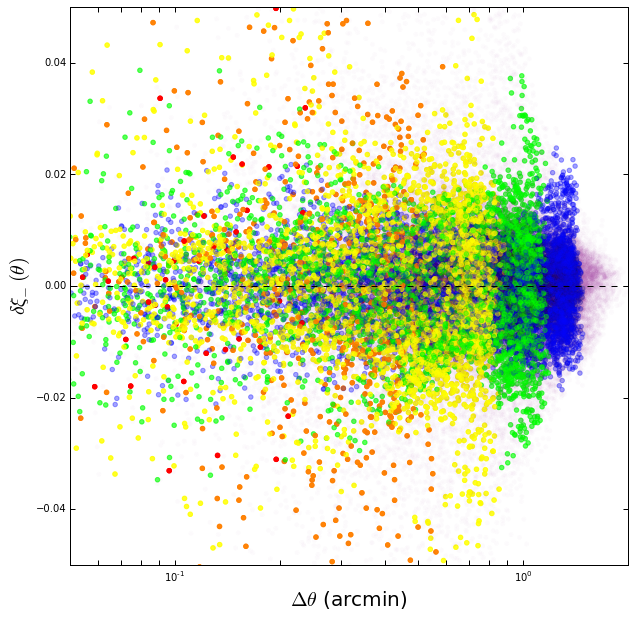
\includegraphics[width=\textwidth]{figs-swe/corr_dist_unlensed.png}
        \captionsetup{justification=raggedright,singlelinecheck=false}
        \caption{The distribution of correlation pairs from the source ellipticities in Figure \ref{color_corr_unlensed}. If the pair of galaxies are in the same color bin, then the correlation scatter point is colored in the same scheme.}
        \label{corr_dist_unlensed}
    \end{subfigure}
    \caption{Correlation visualization for un-lensed galaxies.}
    \label{colored_corr}
\end{figure}

The same plots for the source galaxies \textit{after lensing} are shown in Figure \ref{colored_corr_lensed}. The source ellipticities have clearly aligned tangentially around the foreground lens in Figure \ref{color_corr_lensed}, and distinct patterns have appeared in the correlation pair distribution for each color bin in Figure \ref{corr_dist_lensed}. First consider a single color bin, such as the blue. Galaxies next to one another are lensed in approximately the same way and thus nearly parallel, leading to a positive correlation at small separation distances in Figure \ref{corr_dist_lensed}. Moving a quarter of the way around the blue circle of galaxies, the lensed ellipticities become perpendicular and have negative correlation. This can be seen as the dip in correlation at `middle' separation distances in \ref{corr_dist_lensed}. Finally for galaxies on opposite sides of the lens, their relative orientation is again parallel and the correlation has returned to positive values. This spike in correlation is clearly visible in the distribution and is shifted to the right for colors further from the lens as the radius of the color bin increases. Averaging all scatter points in discrete separation distance bins, the $\varepsilon$-$\varepsilon$ correlation function will no longer be zero and a detectable signal will remain.

%% Color-Coded Correlation Lensed
\begin{figure}
    \centering
    \begin{subfigure}{0.44\textwidth}
        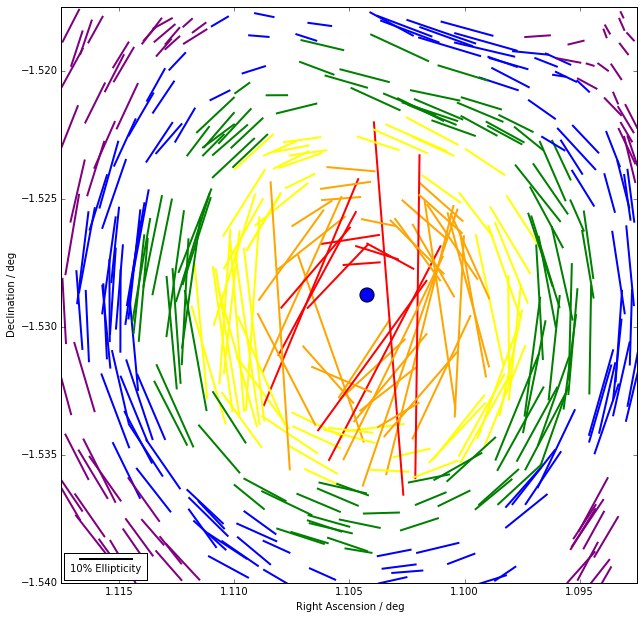
\includegraphics[width=\textwidth]{figs-swe/corr_visualization_lensed.png}
        \captionsetup{justification=raggedright,singlelinecheck=false}
        \caption{The same set of background sources in Figure \ref{color_corr_unlensed} after (magnified for effect) lensing by the foreground mass. Regardless of initial orientation, the source galaxies have all at least partially aligned tangentially around the center lensing mass.}
        \label{color_corr_lensed}
    \end{subfigure}
    ~
    \begin{subfigure}{0.44\textwidth}
        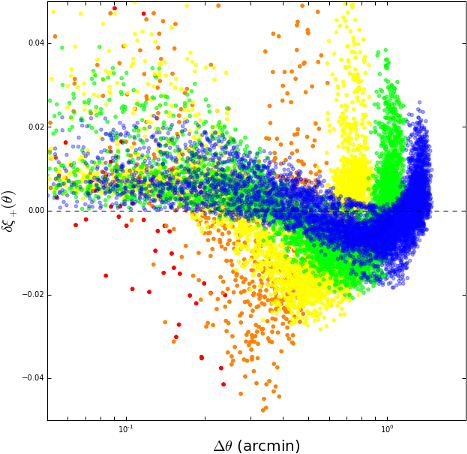
\includegraphics[width=\textwidth]{figs-swe/corr_dist_lensed.png}
        \captionsetup{justification=raggedright,singlelinecheck=false}
        \caption{The distribution of correlation pairs from the source ellipticities in Figure \ref{color_corr_lensed}. If the pair of galaxies are in the same color bin, then the correlation scatter point is colored in the same scheme.}
        \label{corr_dist_lensed}
    \end{subfigure}
    \vspace{-.05in}
    \caption{Correlation visualization for lensed galaxies.}
    \label{colored_corr_lensed}
\end{figure}


%%------------------------------------------------------------------------------------------------------------------------------------------

\newpage

\subsection{Deriving the Standard Correlation Function Definition from \texttt{TreeCorr}'s Definition}

The definition for the shear-shear (or equivalently, in the case of weak lensing, ellipticity-ellipticity) correlation function components in Mike Jarvis's \texttt{TreeCorr} package is different from the common definition given in Equation \eqref{gg_corr_def} from Schneider \cite{schneider}. For the aid of those who wish to use this very useful package but still use the conventional correlation function defintion, I have outlined the connection between the two definitions and the outputs of \texttt{TreeCorr} below:

\setlength\parindent{0pt}

\vspace{0.25 in}

From Jarvis \cite{jarvis} (Page 3):
\begin{align}
\xi_+&=\left<\gamma_i\gamma_j^*\right>=\texttt{xip}+i(\texttt{xip\_im})\label{s+}\\
\xi_-&=\left<\gamma_i\gamma_je^{-4i\alpha}\right>=\texttt{xim}+i(\texttt{xim\_im})\label{s-}
\end{align}

where $\alpha$ is the angle between the two objects $i,j$ and each $\gamma$ is given by $\gamma_n=|\gamma_n|e^{2i\theta_n}$ in polar form.\\

From Schneider \cite{schneider} (Page 92):
\begin{align}
\xi_\pm&=\left<\gamma_{i_t}\gamma_{j_t}\right>\pm\left<\gamma_{i_\times}\gamma_{j_\times}\right>\label{s+-}\\
\xi_\times&=\left<\gamma_{i_t}\gamma_{j_\times}\right>\label{sx}
\end{align}

where $\gamma_{n_t}=-\operatorname{Re}\left(\gamma_n e^{-2i\alpha}\right)$ and $\gamma_{n_\times}=-\operatorname{Im}\left(\gamma_n e^{-2i\alpha}\right)$.\\

\section*{Schneider's $\xi_+$ to Jarvis's \texttt{xip}}

Starting with Schneider's definition, observe that
\begin{align*}
\xi_+&=\left<\gamma_{i_t}\gamma_{j_t}\right>+\left<\gamma_{i_\times}\gamma_{j_\times}\right>\\
&=\left<\operatorname{Re}\left(\gamma_ie^{-2i\alpha}\right)\cdot\operatorname{Re}\left(\gamma_je^{-2i\alpha}\right)\right>+\left<\operatorname{Im}\left(\gamma_ie^{-2i\alpha}\right)\cdot\operatorname{Im}\left(\gamma_je^{-2i\alpha}\right)\right>\\
&=\left<\operatorname{Re}\left(|\gamma_i|e^{2i(\theta_i-\alpha)}\right)\cdot\operatorname{Re}\left(|\gamma_j|e^{2i(\theta_j-\alpha)}\right)\right>+\left<\operatorname{Im}\left(|\gamma_i|e^{2i(\theta_i-\alpha)}\right)\cdot\operatorname{Im}\left(|\gamma_j|e^{2i(\theta_j-\alpha)}\right)\right>\\
&=\left<|\gamma_i|\cdot|\gamma_j|\cos\left(2(\theta_i-\alpha)\right)\cos\left(2(\theta_j-\alpha)\right)\right>+\left<|\gamma_i|\cdot|\gamma_j|\sin\left(2(\theta_i-\alpha)\right)\sin\left(2(\theta_j-\alpha)\right)\right>.
\end{align*}

Using the trig identities
\begin{align}
\cos(u)\cos(v)&=\frac{1}{2}\left[\cos(u-v)+\cos(u+v)\right],\\
\sin(u)\sin(v)&=\frac{1}{2}\left[\cos(u-v)-\cos(u+v)\right],
\end{align}

and the linearity of the expectation operator, it is straightforward to show that
%\begin{align*}
%\xi_+&=\left<|\gamma_i|\cdot|\gamma_j|\right>\cdot\left(\left<\frac{1}{2}\left[\cos\left(2(\theta_i-\theta_j)\right)+\cos\left(2(\theta_i+\theta_j-2\alpha)\right)\right]\right>+\left<\frac{1}{2}\left[\cos\left(2(\theta_i-\theta_j)\right)-\cos\left(2(\theta_i+\theta_j-2\alpha)\right)\right]\right>\right)\\
%&=\left<|\gamma_i|\cdot|\gamma_j|\cos\left(2(\theta_i-\theta_j)\right)\right>.
%\end{align*}
$$\xi_+=\left<|\gamma_i|\cdot|\gamma_j|\cos\left(2(\theta_i-\theta_j)\right)\right>.$$

Now using the identity
\begin{equation}\label{trig2}
\cos(u\pm v)=\cos\left(u\right)\cos\left(v\right)\mp\sin\left(u\right)\sin\left(v\right),
\end{equation}

the previous equation can be written as

\begin{align*}
\xi_+&=\left<|\gamma_i|\cdot|\gamma_j|\cdot\left[\cos\left(2\theta_i\right)\cos\left(2\theta_j\right)+\sin\left(2\theta_i\right)\sin\left(2\theta_j\right)\right]\right>\\
&=\left<\operatorname{Re}(\gamma_i)\cdot\operatorname{Re}(\gamma_j)+\operatorname{Im}(\gamma_i)\cdot\operatorname{Im}(\gamma_j)\right>.
\end{align*}

Using the complex number identities

\begin{align}
\operatorname{Re}(z)&=\frac{1}{2}\left[z+z^*\right],\label{complex1}\\
\operatorname{Im}(z)&=\frac{1}{2i}\left[z-z^*\right]\label{complex2},
\end{align}

it follows that

\begin{align*}
\xi_+&=\left<\frac{1}{4}\left[(\gamma_i+\gamma_i^*)(\gamma_j+\gamma_j^*)-(\gamma_i-\gamma_i^*)(\gamma_j-\gamma_j^*)\right]\right>\\
&=\left<\frac{1}{2}\left[\gamma_i\gamma_j^*+(\gamma_i\gamma_j^*)^*\right]\right>\\
&=\left<\operatorname{Re}(\gamma_i\gamma_j^*)\right>=\texttt{xip}.
\end{align*}

\section*{Schneider's $\xi_-$ to Jarvis's \texttt{xim}}

The first few steps are identical to the previous section besides the negative in the definition of $\xi_-$, giving
\begin{align*}
\xi_-&=\left<\gamma_{i_t}\gamma_{j_t}\right>-\left<\gamma_{i_\times}\gamma_{j_\times}\right>\\
&=\left<|\gamma_i|\cdot|\gamma_j|\cos\left(2(\theta_i-\alpha)\right)\cos\left(2(\theta_j-\alpha)\right)\right>-\left<|\gamma_i|\cdot|\gamma_j|\sin\left(2(\theta_i-\alpha)\right)\sin\left(2(\theta_j-\alpha)\right)\right>\\
&=\left<|\gamma_i|\cdot|\gamma_j|\cos\left(2(\theta_i+\theta_j-2\alpha)\right)\right>.
\end{align*}

Now using Equation \eqref{trig2} twice, first letting $u=2(\theta_i+\theta_j)$ and $v=-4\alpha$, and then letting $u=2\theta_i$ and $v=2\theta_j$, this equation becomes

\begin{align*}
\xi_-&=\left<|\gamma_i|\cdot|\gamma_j|\Big(\left[\cos(2\theta_i)\cos(2\theta_j)-\sin(2\theta_i)\sin(2\theta_j)\right]\cos(4\alpha)+\left[\sin(2\theta_i)\cos(2\theta_j)+\cos(2\theta_i)\sin(2\theta_j)\right]\sin(4\alpha)\Big)\right>\\
&=\Big<\big[\operatorname{Re}(\gamma_i)\cdot\operatorname{Re}(\gamma_j)-\operatorname{Im}(\gamma_i)\cdot\operatorname{Im}(\gamma_j)\big]\cos(4\alpha)+\big[\operatorname{Im}(\gamma_i)\cdot\operatorname{Re}(\gamma_j)+\operatorname{Re}(\gamma_i)\cdot\operatorname{Im}(\gamma_j)\big]\sin(4\alpha)\Big>.
\end{align*}

Using the identities \eqref{complex1} and \eqref{complex2}, and simplifying the leftover terms, this equation can be shown to equal
\begin{align*}
\xi_-=\big<\operatorname{Re}(\gamma_i\gamma_j)\cos(4\alpha)+\operatorname{Im}(\gamma_i\gamma_j)\sin(4\alpha)\big>.
\end{align*}

Now observe that for two complex numbers $a$ and $b$, it is true that

$$\operatorname{Re}(a\cdot b^*)=\operatorname{Re}(a)\cdot\operatorname{Re}(b)+\operatorname{Im}(a)\cdot\operatorname{Im}(b).$$

Then setting $a=\gamma_i\gamma_j$ and $b=e^{4i\alpha}$, it must be true that

$$\operatorname{Re}\left(\gamma_i\gamma_je^{-4i\alpha}\right)=\operatorname{Re}(\gamma_i\gamma_j)\cos(4\alpha)+\operatorname{Im}(\gamma_i\gamma_j)\sin(4\alpha).$$

Combining this with our previous result, this means that

$$\xi_-=\big<\operatorname{Re}(\gamma_i\gamma_j)\cos(4\alpha)+\operatorname{Im}(\gamma_i\gamma_j)\sin(4\alpha)\big>=\left<\operatorname{Re}\left(\gamma_i\gamma_je^{-4i\alpha}\right)\right>=\texttt{xim}.$$

\section*{Schneider's $\xi_\times$ to Jarvis's $\frac{1}{2}\left(\texttt{xim\_im}-\texttt{xip\_im}\right)$}

Starting from Schneider's definition of $\xi_\times$,

\begin{align*}
\xi_\times&=\left<\gamma_{i_t}\gamma_{j_\times}\right>\\
&=\left<\operatorname{Re}\left(|\gamma_i|e^{2i(\theta_i-\alpha)}\right)\cdot\operatorname{Im}\left(|\gamma_j|e^{2i(\theta_j-\alpha)}\right)\right>\\
&=\big<|\gamma_i|\cdot|\gamma_j|\cos\left(2(\theta_i-\alpha)\right)\sin\left(2(\theta_j-\alpha)\right)\big>.\\
\end{align*}

Using the trig identity

\begin{equation}\label{trig3}
\cos(u)\sin(v)=\frac{1}{2}\left[\sin(u+v)-\sin(u-v)\right],
\end{equation}

the previous equation becomes

\begin{align*}
\xi_\times&=\left<|\gamma_i|\cdot|\gamma_j|\cdot\frac{1}{2}\big[\sin\left(2(\theta_i+\theta_j-2\alpha)\right)-\sin\left(2(\theta_i-\theta_j)\right)\big]\right>.
\end{align*}

Next, applying the identities

\begin{equation}\label{trig4}
\sin(u\pm v)=\sin(u)\cos(v)\pm\cos(u)\sin(v)
\end{equation}

along with \eqref{trig2} iteratively until each trig function only has a single term, the equation becomes

\begin{align*}
\xi_\times&=\Big<|\gamma_i|\cdot|\gamma_j|\cdot\frac{1}{2}\Big(\left[\sin(2\theta_i)\cos(2\theta_j)+\cos(2\theta_i)\sin(2\theta_j)\right]\cos(4\alpha)\\
&\qquad\qquad\qquad\quad-\left[\cos(2\theta_i)\cos(2\theta_j)-\sin(2\theta_i)\sin(2\theta_j)\right]\sin(4\alpha)\\
&\qquad\qquad\qquad\quad-\sin(2\theta_i)\cos(2\theta_j)+\cos(2\theta_i)\sin(2\theta_j)\Big)\Big>\\
&=\Big<\frac{1}{2}\Big(\left[\operatorname{Im}(\gamma_i)\cdot\operatorname{Re}(\gamma_j)+\operatorname{Re}(\gamma_i)\cdot\operatorname{Im}(\gamma_j)\right]\cos(4\alpha)\\
&\qquad-\left[\operatorname{Re}(\gamma_i)\cdot\operatorname{Re}(\gamma_j)-\operatorname{Im}(\gamma_i)\cdot\operatorname{Im}(\gamma_j)\right]\sin(4\alpha)\\
&\qquad-\operatorname{Im}(\gamma_i)\operatorname{Re}(\gamma_j)+\operatorname{Re}(\gamma_i)\cdot\operatorname{Im}(\gamma_j)\Big)\Big>.\\
\end{align*}

Using the identities \eqref{complex1} and \eqref{complex2}, this can be simplified to

\begin{align*}
\xi_\times&=\left<\frac{1}{2}\big[\operatorname{Im}(\gamma_i\gamma_j)\cos(4\alpha)-\operatorname{Re}(\gamma_i\gamma_j)\sin(4\alpha)-\operatorname{Im}(\gamma_i\gamma_j^*)\big]\right>.
\end{align*}

Consider again two complex numbers $a$ and $b$. Observe that

$$\operatorname{Im}(a\cdot b^*)=\operatorname{Im}(a)\cdot\operatorname{Re}(b)-\operatorname{Re}(a)\cdot\operatorname{Im}(b).$$

Then setting $a=\gamma_i\gamma_j$ and $b=e^{4i\alpha}$, it must be true that

$$\operatorname{Im}\left(\gamma_i\gamma_je^{-4i\alpha}\right)=\operatorname{Im}(\gamma_i\gamma_j)\cos(4\alpha)-\operatorname{Re}(\gamma_i\gamma_j)\sin(4\alpha).$$

Combing these results give

\begin{align*}
\xi_\times&=\left<\frac{1}{2}\big[\operatorname{Im}(\gamma_i\gamma_j)\cos(4\alpha)-\operatorname{Re}(\gamma_i\gamma_j)\sin(4\alpha)-\operatorname{Im}(\gamma_i\gamma_j^*)\big]\right>\\
&=\left<\frac{1}{2}\big[\operatorname{Im}\left(\gamma_i\gamma_je^{-4i\alpha}\right)-\operatorname{Im}(\gamma_i\gamma_j^*)\big]\right>\\
&=\frac{1}{2}\big[\texttt{xim\_im}-\texttt{xip\_im}\big].
\end{align*}

as desired.

\end{document}
